\documentclass[a4paper,12pt]{report}
\usepackage[left=3cm,right=2.5cm,top=2.5cm,bottom=2.5cm]{geometry}
% \usepackage[left=1.5cm,right=1.5cm,top=2cm,bottom=2cm]{geometry}
\usepackage[T1]{fontenc}
\usepackage[utf8]{inputenc}
\usepackage[english,greek]{babel}
\usepackage{amsmath,amsfonts,amssymb}
\usepackage[parfill]{parskip}
\usepackage[unicode]{hyperref}
\usepackage{bookmark}
\usepackage{cite}
\usepackage{graphicx}
\usepackage{subcaption}
\usepackage{float}
\usepackage{siunitx}
\usepackage{color}
\usepackage{svg}
\usepackage{relsize}
\usepackage{outlines}
\usepackage{kmath,kerkis}
\usepackage{booktabs}
\usepackage{afterpage}

\newcommand\blankpage{%
    \null
    \thispagestyle{empty}%
    \addtocounter{page}{-1}%
    \newpage}

\usepackage{todonotes}
\paperwidth=\dimexpr \paperwidth + 6cm\relax
\oddsidemargin=\dimexpr\oddsidemargin + 3cm\relax
\evensidemargin=\dimexpr\evensidemargin + 3cm\relax
\marginparwidth=\dimexpr \marginparwidth + 3cm\relax

\newcommand{\ra}[1]{\renewcommand{\arraystretch}{#1}}

\graphicspath{{../PICS/}}

\def\tl{\textlatin}
\def\tg{\textgreek}

\begin{document}

\begin{titlepage}

\begin{figure}[H]
  \begin{center}
    
\includegraphics[width=3cm]{auth.pdf}
    \label{fig:cover_auth_logo}
  \end{center}
\end{figure}

\centering
\Large Αριστοτέλειο Πανεπιστήμιο Θεσσαλονίκης\\
\Large Πολυτεχνική Σχολή\\
\large Τμήμα Ηλεκτρολόγων Μηχανικών και Μηχανικών Υπολογιστών\\
\large Τομέας Ηλεκτρονικής και Υπολογιστών

\vspace{\fill}

\LARGE Εκτίμηση ιδιοτήτων εδάφους με χρήση\\
\LARGE δισδιάστατων συνελικτικών νευρωνικών δικτύων
\LARGE και βαθειάς μηχανικής μάθησης

\vspace{\fill}

\Large Διπλωματική Εργασία\\
\Large του\\
\Large Χαράλαμπος Παπαδιάκος

\vspace{\fill}
\raggedright

\begin{tabular}{ll}
\textbf{Επιβλέπων:} & Ιωάννης Θεοχάρης\\
 & Καθηγητής Α.Π.Θ.\\
\end{tabular}

\centering
\vspace{\fill}
\today

\end{titlepage}

\begin{abstract}
Η τεχνητή νοημοσύνη διεισδύει ολοένα και περισσότερο στην καθημερινότητα μας, υποσχόμενη να διευκολύνει το σύνολο της ανθρωπότητας μέσω της απαλλαγής της από χρονοβόρες και απαιτητικές σε ανθρώπινο δυναμικό διαδικασίες ή την διευκόλυνση τους. Ένα πεδίο εφαρμογής της τεχνητής νοημοσύνης το οποίο αναπτύσσεται ραγδαία είναι το \tl{soil spectroscopy}, όπου αποσκοπείται να ελαχιστοποιηθεί η προσπάθεια που απαιτείται για την εξαγωγή των χαρακτηριστικών σε διάφορες εδαφικές ύλες. Ένας μηχανισμός που θα μπορούσε να προβλέψει αυτά τα χαρακτηριστικά με ακρίβεια χρησιμοποιώντας μόνο την φασματική υπογραφή του συγκεκριμένου εδάφους, θα πρόσφερε σίγουρα μια αξιοσημείωτη εναλλακτική, σε σχέση με την απαραίτητη μακροσκελή διαδικασία που απαιτείται κατά την αναλυτική εργαστηριακή μέτρηση των ιδιοτήτων του.\\

Στην παρούσα διπλωματική εργασία γίνεται μια προσπάθεια εκτίμησης χημικών και άλλων ιδιοτήτων του εδάφους ως περαιτέρω ανάλυση πάνω σε ήδη υπάρχουσες υλοποιήσεις για την διεκπεραίωσή του παραπάνω σκοπού με τη χρήση συνελικτικών νευρωνικών δικτύων 2 διαστάσεων.\\

Λόγω της πολύπλοκότητας που φέρει η εφαρμογή μιας αρχιτεκτονικής των συγκεκριμένων δικτύων, γίνεται μια προσπάθεια αύξησης της απόδοσης του συνολικού συστήματος πρόβλεψης, μέσω της ελαχιστοποίησης των παραμέτρων που ορίζουν το μέγεθος του νευρωνικού δικτύου χωρίς ενώ ταυτοχρόνως διατηρειται σε επιθυμητά επίπεδα η τελική επίδοση του.\\

Η υλοποίηση γίνεται στη γλώσσα \tl{Python} με τη χρήση των βιβλιοθηκών \tl{Tensorflow\cite{tensorflow} - Keras\cite{keras}}. Τα πειράματα που πραγματοποιήθηκαν για την εξαγωγή των αποτελεσμάτων έλαβαν χώρο στην ιδρωματική συστοιχία του Α.Π.Θ. ~\cite{hpcauth}
\end{abstract}

\selectlanguage{english}
\begin{abstract}
Artificial Intelligence is becoming more and more a part of our daily life, offering convenient alternatives to time consuming and human resource demanding processes, or providing a helping hand for their conduction. An area of appliance for artificial intelligence that is rapidly growing is soil spectroscopy, aiming to minimize the work that is required to determine the characteristics of variant soil matters. A mechanism that could predict these soil characteristics accurately using only the spectral signature of specific soil is certain to provide a considerable option over tremendous amount of work\\

This diploma thesis regards a procedure of soil property prediction as an extend of existing implementations on the matter, using two-dimensional convolutional neural networks.\\

Due to the the complexity that arises with the application of models of such architecture, it is attempted to increase the efficiency of the whole prediction model, by minimizing parameters that affect the size of the neural network while maintaining it's performance as high as implementable.\\

The implementation is done in Python using the libraries Tensorflow\cite{tensorflow} - Keras\cite{keras}. The conducted tests are made with the help of the Aristotle University of Thessaloniki's High Performance Computing cluster.~\cite{hpcauth}
\end{abstract}

\thispagestyle{empty}

\selectlanguage{greek}

\section*{Ευχαριστίες}
Θα ήθελα να ευχαριστήσω τον υπεύθυνο καθηγητή μου Κ. Θεοχάρη Ιωάννη καθώς και τον υποψήφιο διδάκτορα Νίκο Τσακιρίδη για την πολύτιμη βοήθεια τους στην περάτωση της παρούσας διπλωματικής εργασίας. Επίσης θα ήθελα να ευχαριστήσω την οικογένεια και τους φίλους μου για την υποστήριξη τους στο διάστημα αυτό της εκπόνησης της διπλωματικής εργασίας αλλά και της πορείας μου ως φοιτητής.
\thispagestyle{empty}

\clearpage


\title{\tl{Soil Property Prediction Using 2D Convolutional Neural Networks and Deep Learning Techniques}}
\author{Χαράλαμπος Παπαδιάκος \\
\href{mailto:charaldp@ece.auth.gr}{\tl{charaldp@ece.auth.gr}}}
\maketitle

\tableofcontents
\listoffigures
\listoftables

\chapter{Εισαγωγή}
\label{ch:introduction}

\section{Σχετικά με το έδαφος}
Το έδαφος αποτελεί ένα σημαντικό μέρος του πλανήτη μας, η χρησιμότητα του οποίου φαίνεται στις βασικές ανθρώπινες ανάγκες όπως είναι η επισιτιστική ασφάλεια, η παραγωγή ενέργειας και η κλιματική αλλαγή \cite{vis_near_spectr}.

Η κατάσταση του εδάφους σήμερα είναι σημαντικό να ελέγχεται συστηματικά καθώς έχουν παρατηρηθεί διάφορα φαινόμενα τα οποία το απειλούν και υποβάθμιση και συνακόλουθα χρήζουν εξέτασης. Κάποια από αυτά είναι η διάβρωση του εδάφους το οποίο οδηγεί στην επιδείνωση της ποιότητας του νερού αλλά και την ελάττωσή της σοδειάς η οποία δύναται να εξάγει μια εδαφική περιοχή \cite{world_soil_under_threat}.

Είναι επιθυμητό να μπορούμε να εξετάσουμε την κατάσταση του εδάφους σε πολλά μέρη του πλανήτη καθώς έτσι μπορεί να αναδειχθεί η ιδιομορφία της εκάστοτε περιοχής. Η σύσταση μιας εδαφικής ύλης μπορεί να μας δώσει πληροφορίες σχετικά με κάποιες χρήσιμες ιδιότητες του όπως οι η εδαφική οργανική ύλη, τα μεταλλικά στοιχεία, η υφή, οι θρεπτικές ουσίες, το νερό, το \tl{pH}, και τα βαριά μέταλλα. Οι ιδιότητες αυτές θα μπορούσαν να χαρακτηριστούν ως δείκτες ποιότητας του εδάφους σχετικά με συγκεκριμένες ικανότητες του με τις οποίες μπορεί να δρα ως βάση για τις επίτευξη των βασικών μας αναγκών.

Οι εργαστηριακές αναλύσεις εδαφικών δειγμάτων ήταν πάντα απαραίτητες για την καταγραφή των διακυμάνσεων των ιδιοτήτων και της κατάστασης της ποιότητας του εδάφους. Η δειγματοληψία τους γίνεται όσο πυκνότερα είναι εφικτό να γίνει σε κάθε έκταση της γης, ώστε να καταγράφεται η ιδιομορφία κάθε περιοχής, ενώ ταυτόχρονα να είναι πρακτικά υλοποιήσιμη \cite{soil_spectr}.

Ωστόσο, πέρα από τις εργαστηριακές αναλύσεις δειγμάτων εδάφους θα ήταν προτιμότερη μια μέθοδος ανάκτησης ιδιοτήτων εδάφους για μεγάλες εκτάσεις με μικρότερο κόστος, ούτως ώστε να είναι εφικτή η διαρκής παρακολούθησή του.

\section{Σχετικά με την φασματοσκοπία εδάφους (\tl{Soil Spectroscopy})}
Η ραγδαία ανάπτυξη της τεχνολογίας που παρατηρείται να επέρχεται όλο και περισσότερο στη ζωή μας, δύναται να προσφέρει απλοποιήσεις σε σύνθετες και κοστοβόρες διαδικασίες. Μια από τις περιπτώσεις όπου η τεχνολογία έρχεται για να δώσει μια αποτελεσματική λύση, αφορά την πιθανή χρήση της φασματοσκοπίας εδάφους (\tl{Soil Spectroscopy}).

Η χρήση μηχανισμών εξαγωγής φασματικών υπογραφών εδαφικής ύλης οδήγησε στην δημιουργία βιβλιοθηκών δεδομένων τα οποία αξιοποιούνται συχνά σε βιβλιογραφικές μελέτες και αναλύσεις. Ένα μέρος των σχετικών αναλύσεων δείχνουν πως με την χρήση μηχανικής μάθησης πάνω σε δεδομένα των συγκεκριμένων βιβλιοθηκών δύναται να εξαχθούν αξιόπιστες προβλέψεις σχετικά με τις χημικές ιδιότητες των εδαφικών δειγμάτων.

Το αντικείμενο της διπλωματικής εργασίας αφορά την επίλυση ενός προβλήματος παλινδρόμησης με τη χρήση συνελικτικών νευρωνικών δικτύων πάνω σε δεδομένα φασματοσκοπίας εδάφους (\tl{Soil Spectroscopy}).

Αρχικά οφείλεται να γίνει μια αναφορά στην τεχνολογία της φασματοσκοπίας εδάφους. Η συγκεκριμένη μέθοδος αποσκοπεί στην εξαγωγή χρήσιμης πληροφορίας σχετικά με εδαφικά δείγματα χρησιμοποιώντας την αλληλεπίδραση τους με ακτινοβολίες, έτσι εξετάζεται η αποφυγή μιας αναλυτικής μελέτης των χημικών ιδιοτήτων και συστατικών του εδάφους. Το αποτέλεσμα από την μέτρηση της ανακλώμενης ακτινοβολίας σε ένα εύρος μηκών κύματος αποτελεί ουσιαστικά την φασματική υπογραφή τους. Για την εξαγωγή των παραπάνω συνήθως χρησιμοποιούνται μήκη κύματος εύρους 350–2500 \tl{nm (Vis-near)} ή και 2500–25,000 \tl{nm (mid-infrared)}.

\section{Στόχοι της διπλωματικής εργασίας}
Οι στόχοι της διπλωματικής εργασίας είναι η μελέτη της μεθόδου κατασκευής δισδιάστατων νευρωνικών δικτύων για την εκτίμηση ιδιοτήτων εδάφους, δηλαδή ενός προβλήματος παλινδρόμησης. Τα δεδομένα το οποία χρησιμοποιούνται είναι από την εδαφική βάση \tl{LUCAS Soil} \cite{lucas_soil}. Κατά την μελέτη μιας ήδη υπάρχουσας υλοποίησης γίνεται μια προσπάθεια για την εύρεση μοντέλων τα οποία έχουν απλούστερη αρχιτεκτονική έτσι η εκπαίδευση τους να μην είναι ιδιαίτερα απαιτητική, ενώ ταυτόχρονα αποσκοπείται μια αξιόλογη επίδοση του μοντέλου στην ικανότητα πρόβλεψης των ιδιοτήτων εδάφους. Κατά την διαδικασία εύρεσης των βέλτιστων παραμέτρων του μοντέλου εξετάζονται ορισμένοι μετασχηματισμοί στο σήμα εισόδου.

\section{Διάρθρωση της διπλωματικής}

Στο κεφάλαιο \ref{ch:lucas_soil} γίνεται μια αναφορά στην εδαφική βάση του \tl{LUCAS} και στις υπάρχουσες τεχνικές οι οποίες έχουν εφαρμοστεί για την επίλυση του προβλήματος της φασματοσκοπίας εδάφους. Κατόπιν, το κεφάλαιο \ref{ch:theoreteical_background} αναλύει το θεωρητικό υπόβαθρο το οποίο είναι απαραίτητο για την εφαρμογή των τεχνικών που προτείνονται για την επίλυση του προβλήματος στη συγκεκριμένη διπλωματική εργασία. Έπειτα στο κεφάλαιο \ref{ch:implementation_method} παρουσιάζεται η μέθοδος υλοποίησης που ακολουθήθηκε καθώς και αναφέρονται οι πιθανοί παράμετροι οι οποίοι πρέπει να βελτιστοποιηθούν. Στο κεφάλαιο \ref{ch:experiments_and_results} δείχνονται τα αποτελέσματα που προκύπτουν από την εφαρμογή της υλοποίησης καθώς, ενώ επίσης γίνεται και μια σύγκριση τους με τα αποτελέσματα της προτεινόμενης υλοποίησης. Τέλος στο κεφάλαιο \ref{ch:conclusions} αναφέρονται τα συμπεράσματα που προέκυψαν από την ανάλυση του θέματος της διπλωματικής εργασίας και των πειραμάτων της και προτείνονται ορισμένες επεκτάσεις οι οποίες θα μπορούσαν να αναλυθούν περαιτέρω.
\chapter{Η εδαφική βάση \tl{LUCAS-Soil} }

\section{Σχετικά με το σετ δεδομένων}
Η βάση εδαφικών δειγμάτων \tl{LUCAS-Soil (Land Use/Cover Area frame statistical Survey Soil)} αποτελεί μια από τις μεγαλύτερες και διαρκώς αναπτυσσόμενες βάσεις εδαφικών δεδομένων. Τα δείγματα της έχουν συγκεντρωθεί από διάφορες περιοχές της Ευρώπης. 
Τα δεδομένα της συγκεκριμένης βάσης χωρίονται σε 2 βασικές κατηγορίες, τα δείγματα \tl{Mineral} και \tl{Organic}. Τα δείγματα της κατηγορίας \tl{Mineral} αποτελούνται από 3 κύριες υποκατηγορίες εδάφους \tl{Grassland, Woodland, Cropland}. Η ποικιλία στις κατηγορίες των εδαφικών δειγμάτων προσφέρει ένος εύρος των χαρακτηριστικών τους όσων αφορά την ορυκτολογία, την υφή, τον σίδηρο και την περιεκτικότητά τους σε ανθρακικό ασβέστιο \cite{nocita_lucas_soil}. Αυτό καθιστά την εδαφική βάση ικανή για την εκτέλεση πειραμάτων τα οποία μπορούν να πραγματοποιούνται προβλέψεις ιδιοτήτων γενικευμένων ειδών εδάφους.

Τα δεδομένα εδάφους που χρησιμοποιούνται στην παρούσα διπλωματική εργασία έχουν υποστεί μια επεξεργασία, καθώς ορισμένα από τα δείγματα του σετ δεδομένων τα οποία έχουν εξωκείμενες τιμές για βασικές ιδιότητες τους όπως ο οργανικός άνθρακας (~200 - 586.8 $g~C~kg^{-1}$), έχουν αφαιρεθεί καθώς η συμβολή τους κατά την εκπαίδευση μοντέλων και την εξαγωγή μετρικών είναι μεγάλη, έτσι δεν είναι εφικτό να εξαχθούν βάσιμα συμπεράσματα σχετικά με τα δεδομένα. Το τελικό πλήθος δειγμάτων που χρησιμοποιούνται είναι περίπου 18000 από τα συνολικά 19000. Τα δείγματα που αφαιρούνται ανήκουν κυρίως στην κατηγορία \tl{Organic}. Ένας ακόμη λόγος που δεν χρησιμοποιείται η συγκεκριμένη κατηγορία είναι πως δεν περιέχει δεδομένα σχετικά με την υφή του εδάφους.

\section{Υπάρχουσες τεχνικές}
Στην υπάρχουσα βιβλιογραφία φαίνεται να έχουν δοκιμαστεί ορισμένες υλοποιήσεις για την ανάλυση των δεδομένων της εδαφικής βάσης του \tl{LUCAS}. Οι υλοποιήσεις που εφαρμόστηκαν εξετάζουν διάφορα είδη μοντέλων μηχανικής μάθησης για παλινδρόμηση. Επίσης αναλύονται οι επιμέρους υποκατηγορίες των δειγμάτων εδάφους ενώ δοκιμάζονται ορισμένες τεχνικές προ-επεξεργασίας των δεδομένων εισόδου ή εφαρμογής μετασχηματισμών σε αυτά.

\subsection{Δημοσίευση του \tl{Stevens A.}}
Στη δημοσίευση του \tl{Stevens A.} \cite{stevens_lucas_soil} αναλύονται τα εδαφικά δείγματα στις κατηγορίες \tl{Mineral} και \tl{Organic} καθώς και τα επιμέρους μέρη της κατηγορίας \tl{Mineral} τα οποία είναι τα \tl{Grassland, Woodland} και \tl{Cropland}. Το μοντέλο πρόβλεψης που χρησιμοποιείται για την παλινδρόμηση είναι ένα πολυμεταβλητό μοντέλο. Παρουσιάζονται όλα τα στατιστικά στοιχεία για όλες της ιδιότητες εδάφους της εδαφικής βάσης του \tl{LUCAS}, ενώ η περαιτέρω ανάλυση εστιάζει στην πρόβλεψη της περιεκτικότητας σε οργανικό άνθρακα καθώς θεωρείται το χρησιμότερο στοιχείο.

Στην ανάλυση που πραγματοποιείται εξετάζεται επίσης η χρήση της περιεκτικότητας σε άμμο σαν εξωτερικός προβλέπτης και γίνεται σύγκριση της επίδοσης με την χρήση μόνο φασματικών υπογραφών ή και με την χρήση του εξωτερικού προβλέπτη. Για την επιλογή των βέλτιστων μοντέλων πρόβλεψης ενδείκνυνται διάφορες μεθόδοι προ-επεξεργασίας των δεδομένων εισόδου όπως ο μετασχηματισμός εξομάλυνσης των \tl{Savitzky}--\tl{Golay} \cite{savitzky_golay}, 1η παράγωγος αυτού του μετασχηματισμού αλλά και ο μετασχηματισμός τυπικής κανονικοποιημένης μεταβλητότητας --- \tl{SNV (Standard Normal Variate)}. Η πρόβλεψη των μοντέλων εξετάζεται σε διαφορετικά μέρη των τμημάτων του σετ δεδομένων τα οποία έχουν ομαδοποιηθεί με βάση την περιεκτικότητα τους σε οργανικό άνθρακα.

\subsection{Δημοσίευση του \tl{Nocita M.}}
Μια παρόμοια ανάλυση γίνεται στο άρθρο του \tl{Nocita M.} \cite{nocita_lucas_soil}, όπου αποπειράται η πρόβλεψη του περιεχομένου οργανικού άνθρακα με τη χρήση μοντέλου μερικών ελαχίστων τετραγώνων. Με τη συγκεκριμένη μέθοδο η πρόβλεψη του μοντέλου προκύπτει με τη χρήση των τιμών ενός πλήθους των κοντινότερων γειτόνων---\tl{nearest neighbours}, οπού το κριτήριο γειτνίασης αφορά την ομοιότητα σε στοιχεία του φάσματος του εκαστοτε εδαφικού δείγματος.

Οι προβλέψεις των μοντέλων χωρίζονται σε 4 διαφορετικά τμήματα της εδαφικής βάσης του \tl{LUCAS}, τα \tl{Grassland, Woodland, Cropland} και \tl{Organic}. Έπειτα από την δοκιμή διαφόρων μεγεθών του αριθμού κοντινότερων γειτόνων προκύπτει η βέλτιστη επίδοση με τη χρήση ενός πλήθους 250 γειτόνων για τα μοντέλα κάθε διαφορετικής κατηγορίας εδάφους.

\subsection{Δημοσίευση του \tl{Padarian J.}}
Μια πιο πρόσφατη προσέγγιση η οποία εξετάζει διεξοδικά τις σημαντικότερες από τις ιδιότητες του εδάφους και είναι το επίκεντρο της παρούσας διπλωματικής εργασίας, είναι η δημοσίευση του \tl{Padarian J.} \cite{padarian_lucas_soil}. Στη συγκεκριμένη μέθοδο γίνεται η χρήση δισδιάστατου νευρωνικού δικτύου, όπου το δισδιάστατο σήμα εισόδου προκύπτει από το μετασχηματισμό \tl{wavelet} του φάσματος ανακλαστικότητας και αποτελεί ουσιαστικά ένα σπεκτρόγραμμα του. Το μοντέλο που προτείνεται αποτελείται από πολλαπλά συνελικτικά επίπεδα, καθώς και επίπεδα συγκέντρωσης μεγίστων και πυκνά συνδεδεμένων επιπέδων.

Η πρόβλεψη των ιδιοτήτων εδάφους της βάσης του \tl{LUCAS} εστιάζει στην περιεκτικότητα οργανικού άνθρακα, την ικανότητα ανταλλαγής κατιόντων, περιεκτικότητα σε πηλό, άμμο, το \tl{pH} και το άζωτο. Για κάθε μία από τις 6 αυτές ιδιότητες δημιουργείται ένα μοντέλο μιας εξόδου, παράλληλα εξετάζεται η επίδοση ενός μοντέλου με παρόμοια αρχιτεκτονική το οποίο όμως έχει πολλές εξόδους. Η σύγκρισή των 2 παραπάνω ειδών μοντέλων γίνεται μαζί με μοντέλα μερικών ελαχίστων τετραγώνων και \tl{Cubist} με καλύτερο από αυτά το μοντέλο πολλών εξόδων. Ωστόσο παρατηρείται πως η επίδοση του μοντέλου πολλών εξόδων απαιτεί ένα ένα επαρκές μέγεθος για το σετ δεδομένων εκπαίδευσης έτσι η επίδοση του είναι χειρότερη σε μια δοκιμή με χρήση ενός μικρότερου σετ δεδομένων.

\chapter{Θεωρητικό υπόβαθρο}
\label{ch:theoreteical_background}

\section{Νευρωνικά δίκτυα}
Το νευρωνικό δίκτυο με την αφηρημένη έννοια του είναι μια δομή η οποία θα μπορούσε να χαρακτηριστεί ως ένας μηχανισμός αριθμητικών πράξεων με συνήθως περισσότερες από μια εισόδους και μια ή περισσότερες εξόδους. Ένα νευρωνικό δίκτυο αποτελείται από τους κόμβους--νευρώνες του (\tl{\textbf{nodes}}) οι οποίοι ενώνονται μέσω των συνάψεων του. Το σύνολο των κόμβων οι οποίοι συνδέονται με τις ίδιες ομάδες συνάψεων λέγεται επίπεδο (\tl{\textbf{layer}}).

Η στατική μορφή ενός νευρωνικού δικτύου ως μηχανισμό εξαγωγής αποτελεσμάτων αριθμητικών πράξεων ή αλλιώς η πρόβλεψη ενός μοντέλου αποτελεί μια απλή διαδικασία όπου το αποτέλεσμα κάθε κόμβου πολλαπλασιάζεται με τα βάρη των συνάψεων και εισέρχεται στους κόμβους του επόμενου επιπέδου σαν είσοδος. Ο συγκεκριμένος μηχανισμός ενός νευρωνικού δικτύου ονομάζεται διάδοση προς τα εμπρός (\tl{\textbf{forward propagation}}).

Ένας ακόμη σημαντικός μηχανισμός που κάνει ένα νευρωνικό δίκτυο ένα χρήσιμο εργαλείο είναι αυτός που δίνει τη δυνατότητα τροποποίησης των βαρών του με αποτέλεσμα την εκπαίδευση του μοντέλου. Ο τρόπος με τον οποίο το παραπάνω είναι εφικτό είναι με μια αντίστροφη διαδικασία από την διάδοση προς τα εμπρός, δηλαδή με βάση μια επιθυμητή τιμή εξόδου τα βάρη του μοντέλου προσαρμόζονται από τα τελευταία προς τα πρώτα επίπεδα, με σκοπό να μειωθεί το σφάλμα ως προς την επιθυμητή έξοδο. Η διαδικασία αυτή ονομάζεται οπισθοδιάδοση \tl{(\textbf{backpropagation})}.

\begin{figure}[H]
  \begin{center}
    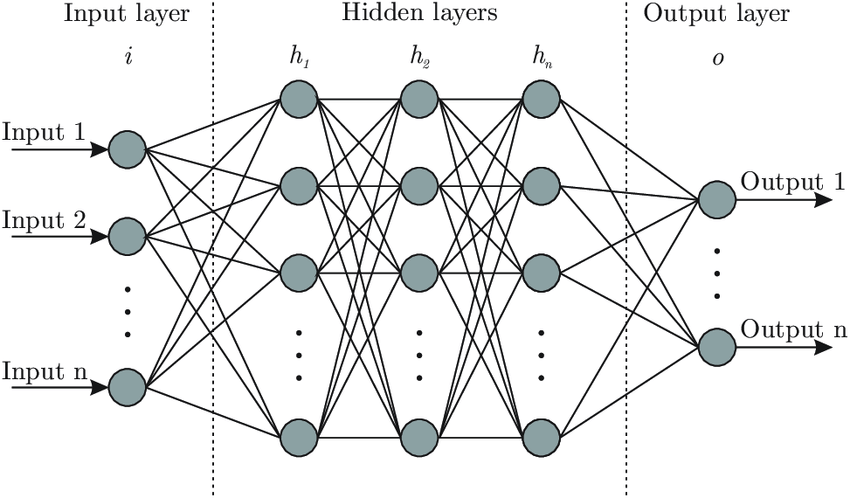
\includegraphics[width=0.8\textwidth]{THEORETICAL_BACKGROUND/neural_network.png}
    \caption{Γενική μορφή Νευρωνικού δικτύου (Πηγή: \href{https://mc.ai/my-notes-on-neural-networks-2/}{\tl{mc.ai}})}
    \label{fig:neur_net}
  \end{center}
\end{figure}

Για τη σωστή λειτουργία ενός νευρωνικού δικτύου είναι απαραίτητοι ορισμένοι επιπλέον μηχανισμοί οι οποίοι μετασχηματίζουν τις τιμές εξόδου των κόμβων --- αυτές είναι οι συναρτήσεις ενεργοποίησης. Μια από τις συναρτήσεις ενεργοποίησης οι οποίες χρησιμοποιούνται συνήθως είναι η ανορθωμένη γραμμική συνάρτηση.

\subsubsection{Ανορθωμένη γραμμική συνάρτηση \tl{(ReLU)}}
Η ανορθωμένη γραμμική συνάρτηση \tl{ReLU (Rectified Linear Unit)} είναι ουσιαστικά η γραμμική συνάρτηση $\mathit{\mathbf{f\left(x\right) = x}}$, η οποία είναι τροποποιημένη στο μέρος της αρνητικής εισόδου της ώστε να μηδενίζει την έξοδο. Η χρήση της είναι συνήθης στην δομή των νευρωνικών δικτύων ως συνάρτηση ενεργοποίησης, λόγω της ιδιότητας της να αποκόπτει αρνητικές τιμές κατά την διάδοση των σημάτων μεταξύ των κόμβων--νευρώνων, κάτι που επιτρέπει την ομαλή εκπαίδευση του.

\begin{figure}[H]
  \begin{center}
    \includesvg[width=1\textwidth]{THEORETICAL_BACKGROUND/ReLU}
    \caption{Μορφή της συνάρτησης ανορθωμένης γραμμικής συνάρτησης \tl{ReLU}}
  \end{center}
\end{figure}

\section{Συνελικτικά Νευρωνικά Δίκτυα}
Τα Συνελικτικά Νευρωνικά Δίκτυα αποτελούν μια συγκεκριμένη μορφή των νευρωνικών δικτύων τα οποία περιλαμβάνουν επίπεδα στα οποία οι κόμβοι δεν είναι πλήρως συνδεδεμένοι με κάθε κόμβο του επομένου επιπέδου αλλά είναι μόνο με ορισμένους που ανήκουν σε μια περιοχή.

Επίσης χρησιμοποιούνται ορισμένοι ακόμη τύποι επιπέδων όπως για παράδειγμα την τροποποίηση των διαστάσεων της εισόδου με συγκέντρωση μεγίστων (\tl{\textbf{Max Pooling}}).

Στις επόμενες υποενότητες θα αναλυθούν τα επιμέρους τμήματα που χρησιμοποιούνται σε ένα συνελικτικό νευρωνικό δίκτυο.

\section{Διαδικασία εκπαίδευσης συνελικτικού νευρωνικού δικτύου}
Κατά την εκπαίδευση ενός συνελικτικού νευρωνικού δικτύου γίνεται χρήση του αλγορίθμου οπισθοδιάδοσης, έτσι το σφάλμα που παρατηρείται στην έξοδο χρησιμοποιείται για την ρύθμιση των βαρών των πλήρως συνδεδεμένων επιπέδων, ενώ στη συνέχεια καθώς η διόρθωση των βαρών των επιπέδων κινείται προς τα πρώτα επίπεδα, ρυθμίζονται οι τιμές των παραμέτρων των συνελικτικών φίλτρων των αντίστοιχων επιπέδων για όλο το σύνολο των φίλτρων που περιλαμβάνουν.\\

Ο ρυθμός τροποποίησης των βαρών κάθε επιπέδου είναι επιθυμητό να γίνεται με έναν τρόπο κατά τον οποίο το συνελικτικό νευρωνικό δίκτυο θα εκπαιδεύεται με ικανοποιητικό ρυθμό, ώστε να μην υπάρχει υποεκπαίδευση. Ωστόσο επιπλέον η μεταβολή των βαρών δεν πρέπει να γίνεται πολύ γρήγορα ειδάλλως υπάρχει ταλάντωση στο σφάλμα εκπαίδευσης και είναι πιθανό να μην μπορεί να συγκλίνει σε κάποιο ελάχιστο σημείο. Με βάση τα παραπάνω φαίνεται πως απαιτείται ένας μηχανισμός ο οποίος θα επιβλέπει τον ρυθμό μεταβολής των βαρών τόσο κατά την εκκίνηση της εκπαίδευσης όσο και στην εξέλιξη της, οι μηχανισμοί αυτοί ονομάζονται βελιστοποιητές \tl{Optimizers} και θα αναλυθούν στη συνέχεια αυτού του κεφαλαίου.

\subsection{Δισδιάστατα Συνελικτικά Επίπεδα}
Τα δισδιάστατα συνελικτικά νευρωνικά δίκτυα είναι γνωστά για τις εφαρμογές τους οι οποίες είναι σχετικές με την εικόνα. Μια συνήθης χρήση των συνελικτικών νευρωνικών δικτύων είναι η ταξινόμηση εικόνων με βάση το αν περιλαμβάνουν ένα συγκεκριμένο αντικείμενο. Μια ακόμη χρήση είναι η αναγνώριση προσώπου, δηλαδή η εξαγωγή χαρακτηριστικών του προσώπου με σκοπό την ταυτοποίηση ενός ατόμου. Παρόμοια είναι επίσης η εφαρμογή της αναγνώρισης των χαρακτηριστικών γραφής.\\

Η είσοδος που χρησιμοποιείται στο μοντέλο πρόβλεψης αυτής της διπλωματικής εργασίας είναι ένα σπεκτρόγραμμα το οποίο είναι είσοδος 2 διαστάσεων, σε αντίθεση με άλλες υλοποιήσεις στις οποίες χρησιμοποιείται συνελικτικό νευρωνικό δίκτυο με είσοδο το φάσμα το οποίο είναι ένα μονοδιάστατο σήμα.\\

Τα συνελικτικά επίπεδα είναι το χαρακτηριστικό μέρος των συνελικτικών δικτύων, όπως προδίδει το όνομα τους αποτελούν τμήματα τα οποία μετασχηματίζουν και εξάγουν από την είσοδο πληροφορία με βάση την εφαρμογή συνελικτικών φίλτρων. Η διαδικασία αυτή επιτρέπει την εξαγωγή χρήσιμης πληροφορίας προς τα επόμενα επίπεδα για την ανίχνευση πιθανών μοτίβων ενώ ταυτόχρονα δεν απαιτεί το μέγεθος των πυκνών \tl{dense} επιπέδων καθώς αφορά πράξεις ενός σημείου της εισόδου με ορισμένα γειτονικά σημεία και όχι την μέθοδο πράξεων σημεία όλα προς όλα.

Η μορφή της περιοχής των γειτονικών σημείων καθορίζεται από το φίλτρο \tl{\textbf{Kernel}} που χρησιμοποιείται. Ο πυρήνας που χρησιμοποιείται συνήθως σε δισδιάστατα νευρωνικά δίκτυα είναι διαστάσεων $3\times3$. Ορισμένες ακόμη παράμετροι των πυρήνων είναι ο αριθμός των φίλτρων που υπάρχουν στο συγκεκριμένο επίπεδο αλλά και ο τρόπος που εφαρμόζονται τα συνελικτικά φίλτρα. Η πρώτη παράμετρος είναι το βήμα συνέλιξης ως προς τις 2 διαστάσεις, το οποίο συνήθως είναι μονάδα, ενώ για τιμές μεγαλύτερες της μονάδας υπάρχει υποδειγματοληψία για το επόμενο επίπεδο. Επίσης κατά την εφαρμογή συνελικτικών φίλτρων υπάρχει η επιλογή συνέλιξης στα άκρα του δισδιάστατου επιπέδου ώστε το συνελικτικό φίλτρο να χωράει πάντα μέσα στην εικόνα, ή η επιλογή συνέλιξης και σε ορισμένα σημεία εκτός της εικόνας με την προσθήκη μηδενκών ώστε το αποτέλεσμα της συνέλιξης να έχει ίδιες διαστάσεις με την αρχική εικόνα.

Κατά την εφαρμογή ενός συνελικτικού επιπέδου στην είσοδο ή οποιοδήποτε ενδιάμεσο επίπεδο, κάθε συνελικτικό φίλτρο εφαρμόζεται σε όλη την έκταση της εικόνας σύμφωνα με τις παραμέτρους βήματος και την επιλογή για τα ακραία σημεία της εικόνας. Το αποτέλεσμα είναι μια εικόνα ίσων ή μικρότερων διαστάσεων και αριθμού καναλιών $\mathbf{N\times M}$ όπου $\mathbf{N}$ ο αριθμός των καναλιών της εικόνας εισόδου και $\mathbf{M}$ ο αριθμός των φίλτρων του συνελικτικού επιπέδου. Ο αριθμός των παραμέτρων εκπαίδευσης του συνελικτικού επιπέδου είναι ίσος με $\mathbf{\left(A \times B\times N+1\right)\times M}$ όπου $\mathbf{A}$ και $\mathbf{B}$ το πλάτος και ύψος του κάθε συνελικτικού φίλτρου.\\

Στην υλοποίηση που εξετάζεται χρησιμοποιούνται συνελικτικά επίπεδα 2 διαστάσεων καθώς η είσοδος του δικτύου όπως θα αναφερθεί προκύπτει ως εικόνα ενός καναλιού έπειτα από μετασχηματισμό του αρχικού σήματος.

\subsection{Πλήρως συνδεδεμένα επίπεδα}
Η χρήση των πλήρως συνδεδεμένων επιπέδων είναι απαραίτητη για την αποτελεσματική πρόβλεψη ενός συνελικτικού νευρωνικού δικτύου. Η τοποθέτηση τους στην δομή του μοντέλου ωστόσο προτιμάται να γίνεται σε σημεία όπου η διαστάσεις του προηγούμενου επιπέδου είναι σχετικά μικρές και η επεξεργασία του συγκεκριμένου επιπέδου αφορά την εκτίμηση της προηγουμένως επεξεργασμένης εισόδου. Η μορφή ενός πλήρως συνδεδεμένου επιπέδου είναι αυτή των κρυφών (\textbf{\tl{Hidden}}) επιπέδων του σχήματος \ref{fig:neur_net}.

Στην αρχιτεκτονική των νευρωνικών δικτύων που πραγματεύεται η παρούσα εργασία τα πλήρως συνδεδεμένα επίπεδα τοποθετούνται μετά από τα συνελικτικά επίπεδα και ακριβώς πριν την έξοδο.

\subsection{Επίπεδα κανονικοποίησης παρτίδας(\tl{Batch Normalization})}
Η χρησιμότητα των επιπέδων κανονικοποίησης παρτίδας είναι στην εκπαίδευση των νευρωνικών και έχει ως σκοπό την αποφυγή της συνδιακυμαίνουσας μετατόπισης. Η συνδιακυμαίνουσα μετατόπιση είναι ένα φαινόμενο που οφείλεται στις τροποποιήσεις των παραμέτρων των συνελικτικών επιπέδων με αποτέλεσμα την διακύμανση των εξόδων τους.\\

Κατά την κανονικοποίηση παρτίδας τα δεδομένα τα οποία χρησιμοποιούνται κατά την εκπαίδευση μέσα σε μια εποχή χωρίζονται σε ομάδες ορισμένου μεγέθους το οποίο ονομάζεται μέγεθος παρτίδας (\tl{Batch Size}). Για κάθε παρτίδα τα δεδομένα κανονικοπούνται πριν από τις συναρτήσεις ενεργοποίησης των συνελικτικών και πλήρως συνδεδεμένων επιπέδων ώστε να έχουν μέση τιμή μηδέν και διακύμανση μονάδα.

Ένα βασικό όφελος που προκύπτει από την χρήση της κανονικοποίηση παρτίδας, είναι η επιτάχυνση της διαδικασίας της εκπαίδευσης μέσω της παράλληλης επεξεργασίας των δειγμάτων με την χρήση της κάρτας γραφικών ενός υπολογιστικού συστήματος.

\subsection{Επίπεδα \tl{Dropout}}
Η μέθοδος \tl{Dropout} αποσκοπεί σε μια πιο εύρωστη εκπαίδευση ενός νευρωνικού δικτύου. Ο τρόπος με τον οποίο λειτουργεί είναι με την τυχαία απενεργοποίηση νευρώνων με αποτέλεσμα την αναγκαστική εκπαίδευση εναλλακτικών νευρώνων, δηλαδή αποφεύγεται η υπερενεργοποίηση συγκεκριμένων νευρώνων για συγκεκριμένες εισόδους όπως επίσης και η αδρανοποίηση ορισμένων νευρώνων οι οποίοι ενδεχομένως να ήταν πιο "τεμπέλικοι" εάν δεν χρησιμοποιούνταν η συγκεκριμένη τεχνική.

\subsection{Επίπεδα υποδειγματοληψίας --- Συγκέντρωση μεγίστων \tl{(Max Pooling)}}
Τα επίπεδα υποδειγματοληψίας είναι σημαντικά για τη δομή ενός συνελικτικού νευρωνικού δικτύου καθώς μειώνουν τις διαστάσεις την διάσταση της εισόδου μειώνοντας έτσι τον αριθμό των παραμέτρων του νευρωνικού δικτύου. Ταυτόχρονα η πληροφορία από τα σημεία της εισόδου που έχουν ενεργοποιηθεί δεν χάνεται. 

Κατά την εφαρμογή ενός επιπέδου συγκέντρωσης ορίζεται μια περιοχή συγκέντρωσης από τις τιμές της εισόδου σε αυτή την περιοχή θα εξαχθεί μια τιμή ανάλογα με τον τύπο επιπέδου συγκέντρωσης. Η διάσταση της περιοχής συγκέντρωσης είναι συνήθως $2\times2$. 

\begin{figure}[H]
  \begin{center}
    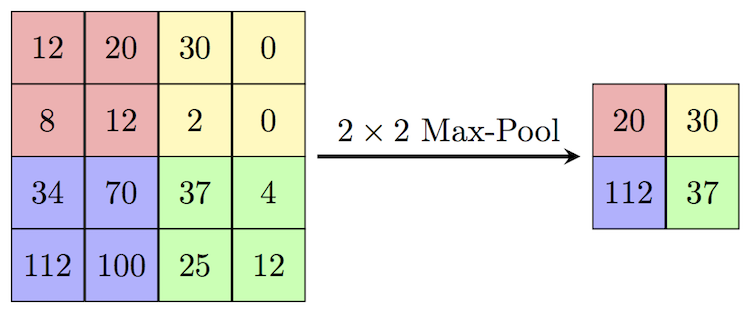
\includegraphics[width=0.7\textwidth]{THEORETICAL_BACKGROUND/max_pooling.png}
    \caption{Μέθοδος συγκέντρωσης μεγίστων για περιοχές διαστάσεων $2\times2$ (Πηγή: \href{https://computersciencewiki.org/index.php/Max-pooling_/_Pooling}{\tl{Computer Science Wiki}})}
  \end{center}
\end{figure}

Οι 2 τύποι επιπέδων υποδειγματοληψίας είναι τα συγκέντρωσης μεγίστων και συγκέντρωσης μέσης τιμής. Στην υλοποίηση που χρησιμοποιήθηκε παρατηρήθηκε πως η χρήση συγκέντρωσης μεγίστων έχει σημαντικά καλύτερη επίδοση σε σχέση με την συγκέντρωση μέσου όρου.

\subsection{Αρχικοποίηση Νευρωνικών Δικτύων}
Κατά την αρχικοποίηση ενός νευρωνικού δικτύου, η εκχώρηση των κατάλληλων βαρών των τεχνητών νευρώνων κάθε κόμβου παίζει σημαντικό ρόλο στην μετέπειτα δυνατότητα του μοντέλου να έχει μια στατιστικά αμερόληπτη κατάσταση εκκίνησης της εκπαίδευσης του, έτσι είναι εφικτό να τροποποιούνται τα βάρη του με κατάλληλο τρόπο ώστε να βελτιώνεται η απόδοση του κατά την διαδικασία της εκπαίδευσης.
Για τον παραπάνω σκοπό υπάρχουν ορισμένες μέθοδοι αρχικοποίησης των βαρών ενός μοντέλου
Ένας από του αρχικοποιητές που χρησιμοποιήθηκε για τα συνελικτικά φίλτρα είναι ο \tl{kernel\_initializer *random\_uniform*}. Οι αρχικές τιμές με τη χρήση του παραπάνω προκύπτουν από μια ομοιόμορφη κατανομή ενός ορισμένου εύρους τιμών. Η αρχικοποίηση των διανυσμάτων πόλωσης έγινε με τη χρήση του αρχικοποιητή
 \tl{bias\_initializer: zeros}, όπου οι αρχικές τιμές του διανύσματος πόλωσης ορίζονται μηδέν.

\subsection{Μέθοδοί ελαχιστοποίησης σφάλματος --- Βελτιστοποιητές \tl{(Optimizers)}}
Όπως προαναφέρθηκε η χρήση ενός μηχανισμού τροποποίησης του ρυθμού εκμάθησης και επίβλεψης του σφάλματος εκπαίδευσης είναι απαραίτητος για την επιτυχή εκπαίδευση ενός μοντέλου. 

\subsubsection{Στοχαστική κατάβαση δυναμικού \tl{SGD (Stochastic Gradient Descent)}}
Η πιο γνωστή μέθοδος ελαχιστοποίησης σφάλματος είναι η στοχαστική κατάβαση δυναμικού \tl{\textbf{SGD (Stochastic Gradient Descent)}}, η οποία αποτελεί μια απλή μέθοδο για την ελαχιστοποίηση του σφάλματος με βάση μια συνάρτηση σφάλματος η οποία στην περίπτωση των νευρωνικών δικτύων είναι συνήθως ένα άθροισμα των εισόδων ενός επιπέδου πολλαπλασιασμένων με τα βάρη τους. Η τρόπος με τον οποίο πραγματοποιείται η ελαχιστοποίηση της συνάρτησης είναι με τη χρήση της μερικής παραγώγου της ή αλλιώς την κλίση της. Για την μείωση της πολυπλοκότητας του αλγορίθμου η διαδικασία εκτελείται με στοχαστικό τρόπο, δηλαδή οι υπολογισμοί των παραγώγων δεν γίνονται για όλα τα σημεία του σετ δεδομένων αλλά επιλέγονται ορισμένα από αυτά με έναν τυχαίο τρόπο.

\subsubsection{Αλγόριθμος \tl{RMSprop}}
Ο \tl{RMSprop} είναι επίσης ένας γνωστός αλγόριθμος για την χρήση του σε βαθειά μηχανική μάθηση. Έχει ως βάση τον απλοποιημένο αλγόριθμο rprop όπου γίνεται χρήση της κλίσης αλλά και διαίρεση με αυτή έτσι εστιάζει κυρίως στη χρήση του προσήμου αυτής. Ωστόσο επειδή ο \tl{RMSprop} εφαρμόζεται σε μικρές ομάδες δειγμάτων, η υλοποίηση τροποποιείται με τη χρήση ενός κινητού μέσου όρου του τετραγώνου των κλίσεων κάθε βάρους ώστε να μπορεί να χρησιμοποιήθει σε όλα τα δείγματα. Το όνομα του αλγορίθμου προκύπτει από το χαρακτηριστικό του να διαιρεϊται η κλίση με την τετραγωνική ρίζα των μέσων τετραγώνων \tl{RMS}.

\subsubsection{Βελτιστοποιητής \tl{Adam}}
Μια από τις μεθόδους ελαχιστοποίησης σφάλματος η οποία παρατηρήθηκε πως είναι κατάλληλη για την χρήση σε συνελικτικά νευρωνικά δίκτυα είναι ο βελτιστοποιητής \tl{Adam (Adaptive Moment Estimation)}. Θα μπορούσε να θεωρηθεί ως ένας συνδυασμός των \tl{RMSprop} και \tl{SGD}. Ο τρόπος με τον οποίο μοιάζει με αυτούς τους 2 βελτιστοποιητές είναι ότι γίνεται χρήση των τετραγώνων της κλίσης για την κλιμακοποίηση του ρυθμού εκμάθησης όπως στον αλγόριθμο \tl{RMSprop}, ενώ επίσης χρησιμοποιεί το στοιχείο της ορμής με τη εφαρμογή ενός κινούμενου μέσου όρου της κλίσης, κάτι που μοιάζει με τον αλγόριθμο \tl{SGD} με ορμή.\\

Ο υπολογισμός της παραμέτρου 1ης και της 2ης ορμής αντίστοιχα γίνεται με βάση τους παρακάτω τύπους:
$$m_t=\beta_1m_{t-1}+\left(1-\beta_1\right)g_t$$
$$v_t=\beta_2v_{t-1}+\left(1-\beta_2\right)g_t^2$$

\subsubsection{Βελτιστοποιητής \tl{Nadam}}
Ένας ακόμη βελτιστοποιητής που χρησιμοποιείται είναι ο \tl{Nadam} ο οποίος πρόκειται για μια τροποποίηση του \tl{Adam} που συνδυάζει τον αλγορίθμου \tl{NAG (Nesterov accelerated SGD)}. Το χαρακτηριστικό του αλγορίθμου \tl{NAG} είναι πως δεν χρησιμοποιεί το τρέχον βήμα αλλά και το επόμενο, έτσι υπάρχει αξιοσημείωτη ελάττωση των ταλαντώσεων της καμπύλης του σφάλματος με επακόλουθο μια αποτελεσματικότερη εκπαίδευση.\\

\section{Μέθοδος εξαγωγής \tl{Spectrogram}}
Το σπεκτρόγραμμα είναι μια δισδιάστατη αναπαράσταση ενός μονοδιάστατου σήματος όπου στον κατακόρυφο άξονα αποτυπώνεται το φασματικό περιεχόμενο μιας περιοχής του αρχικού σήματος. Η εξαγωγή των σπεκτρογραμμάτων συνήθως χρησιμοποιείται σε σήματα τα οποία είναι συνάρτηση του χρόνου με σκοπό την εξαγωγή χαρακτηρηστικών σχετικά με το φάσμα και την συχνότητα.\\
Για την εξαγωγή ενός σπεκτρογράμματος το αρχικό σήμα χωρίζεται σε ένα πλήθος $K$ τμημάτων με τη χρήση παραθύρων σταθερού μήκους $M$ δειγμάτων, χρησιμοποιώντας επικάλυψη $N$ ανάμεσα σε διαδοχικά παράθυρα. Σε κάθε τμήμα του σήματος στο οποίο έχει εφαρμοστέι η συνάρτηση παραθύρου, γίνεται μετασχηματισμός Fourier μικρής χρονικής διάρκειας \tl{STFT (Short Time Fourier Transform)}. Έτσι το τελικό πλήθος των υποτμημάτων $K$, το οποίο θα είναι και η οριζόντια διάσταση του σπεκτρογράμματος, ορίζεται από την μορφή των παραθύρων αλλά και την επικάλυψη τους.\\
Η οριζόντια διάσταση της μονοκαναλικής εικόνας που προκύπτουν είναι 
$$K=\lfloor\frac{X}{M-K}\rfloor+1$$
Όπου $X$ το συνολικό μήκος του αρχικού μονοδιάστατου σήματος.

\begin{figure}[H]
  \begin{center}
    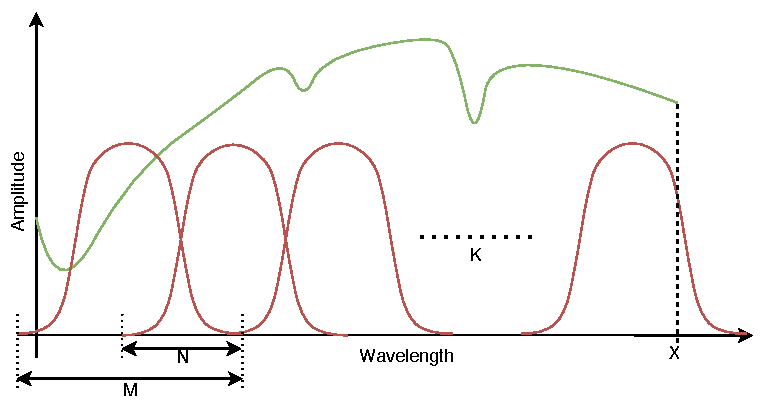
\includegraphics[width=1\textwidth]{THEORETICAL_BACKGROUND/SpectrogramWindows.pdf}
    \caption{Απεικόνιση της μεθόδου εφαρμογής επικαλυπτόμενων παραθύρων σε φασματική υπογραφή}
  \end{center}
\end{figure}

\begin{figure}[H]
    \begin{subfigure}{0.5\textwidth}
        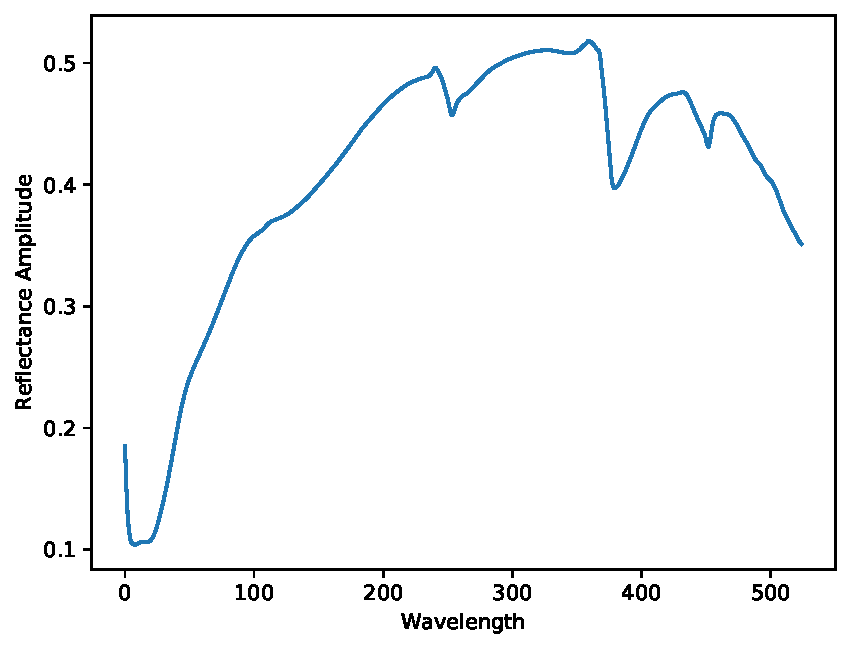
\includegraphics[width=1\textwidth]{THEORETICAL_BACKGROUND/Reflectance.pdf}
    \end{subfigure}
    \begin{subfigure}{0.5\textwidth}
        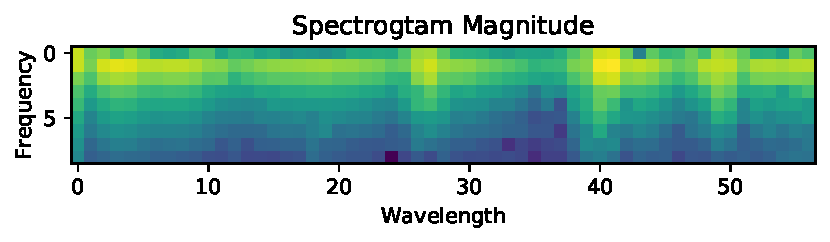
\includegraphics[width=1\textwidth]{THEORETICAL_BACKGROUND/Spectrogram.pdf}
    \end{subfigure}
    \caption{Μορφή της φασματικής υπογραφής πριν και μετά την μετατροπή σε σπεκτρόγραμμα}
\end{figure}

Ο τύπος του παραθύρου που επιλέγεται ορίζει κατά κάποιον τρόπο τον αποτέλεσμα του μετασχηματισμού \tl{STFT}. Τα χαρακτηριστικά που έχει ένα παράθυρο που χρησιμοποιείται για την εξαγωγή σπεκτρογραμμάτων είναι η συμμετρία του ως προς το μέσον του, η ομαλή μετάβαση προς το μηδέν στα άκρα του και μια απόκριση στο φάσμα στην οποία να υπάρχουν κυρίως οι χαμηλότερες συχνότητες ενώ οι υψηλότερες να έχουν σημαντικά μικρότερη τιμή.

\begin{figure}[H]
  \begin{center}%\selectlanguage{english}
    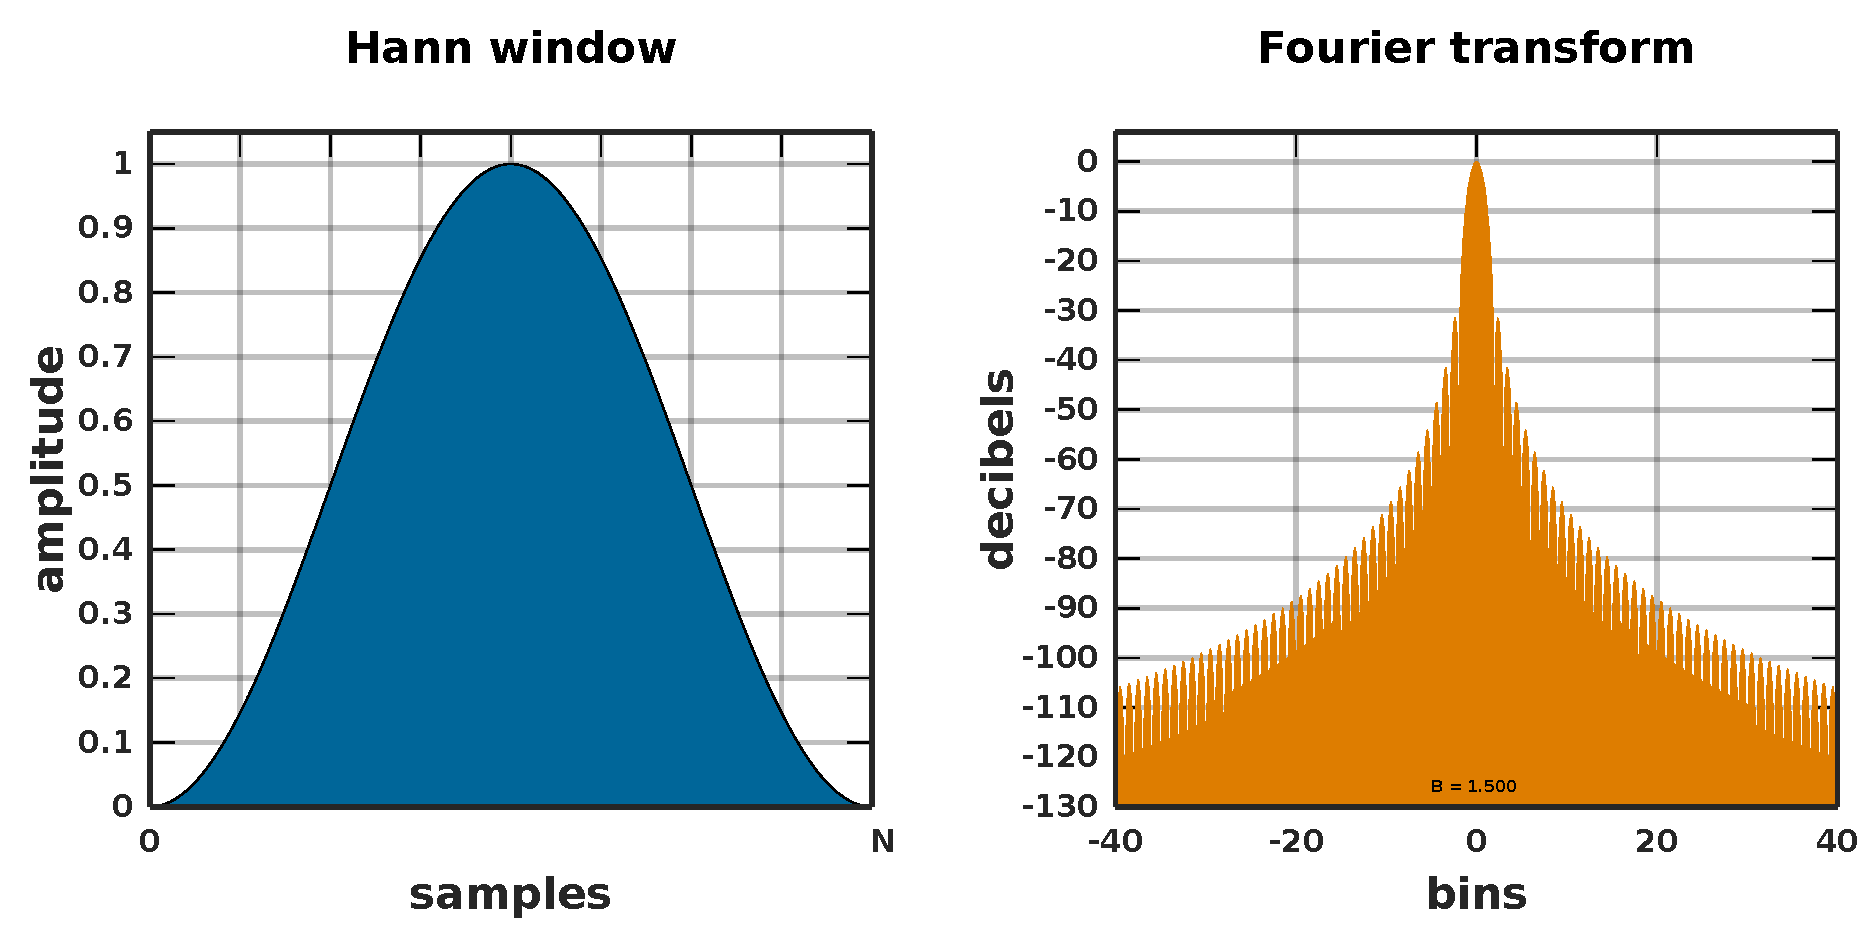
\includegraphics[width=1\textwidth]{THEORETICAL_BACKGROUND/HannWindow.pdf}
    %\selectlanguage{greek}
    \caption{Απόκριση του παραθύρου \tl{Hann} στο χρόνο (αριστερά) και στη συχνότητα (δεξιά)}
  \end{center}
\end{figure}

\section{Μετασχηματισμός των \tl{Savitzky--Golay}}
Ο μετασχηματισμός των \tl{Savitzky--Golay}\cite{savitzky_golay} είναι μια μέθοδος εξομάλυνσης ενός σήματος. Ο τρόπος που εξάγεται είναι ουσιαστικά με τη χρήση μιας συνέλιξης κατά την οποία για κάθε δείγμα με τη χρήση των γειτονικών δειγμάτων του γίνεται εκτίμηση μιας καμπύλης του σήματος με τη χρήση πολυωνύμων μικρού βαθμού. Επίσης είναι μια συχνή στρατηγική ο μετασχηματισμός των tl{Savitzky--Golay} να χρησιμοποιείται για την εξαγωγή μιας εξομαλυσμένης μορφής της 1ης ή της 2ης παραγώγου ενός σήματος.\\

Σχήμα αρχικού---μετασχηματισμένου σήματος

\section{Μετρικές απόδοσης των μοντέλων}
Οι μετρικές αξιολόγησης που χρησιμοποιήθηκαν είναι το μέσο τετραγωνικό σφάλμα, η ρίζα του μέσου τετραγωνικού σφάλματος, ο συντελεστής προσδιορισμού και το ενδοτεραρτημοριακό εύρος. Είναι επιθυμητό κάθε μοντέλο να αξιολογείται με τη χρήση διαφορετικών μετρικών καθώς κάθε μια από αυτές εκφράζουν με ξεχωριστό τρόπο την επίδοση ενός μοντέλου και η χρησιμότητα τους μπορεί να διαφέρει ανάλογα με τις ιδιαιτερότητες της εξόδου που προβλέπεται.

\subsection{Μέσο τετραγωνικό σφάλμα}
Η μετρική του μέσου τετραγωνικού σφάλματος είναι μια από τις πιο συνήθεις για την εκπαίδευση και αξιολόγηση μοντέλων. Η χρησιμότητα της οφείλεται στο γεγονός πως η τετραγωνισμένες τιμές των σφαλμάτων τονίζουν περισσότερο τα μεγαλύτερα σφάλματα πρόβλεψης κάτι το οποίο είναι χρήσιμο κατά την εκπαίδευση. Ο τύπος υπολογισμού είναι ο παρακάτω.

$$MSE=\frac{1}{n}\sum_{i=1}^{n} {\left(x_{i}-\hat{x_{i}}\right)}^2$$

\subsection{Ρίζα του μέσου τετραγωνκού σφάλματος}
Η συγκεκριμένη μετρική είναι σχεδόν ίδια με το μέσο τετραγωνικό σφάλμα με την διαφορά ότι η τιμή της είναι πιο αντιπροσωπευτική ως προς το μέγεθος των τιμών της σε σχέση με τις τιμές της εξόδου.

$$RMSE=\sqrt{\frac{1}{n}\sum_{i=1}^{n} {\left(x_{i}-\hat{x_{i}}\right)}^2}$$
Όπου $\hat{x_{i}}$ είναι η πρόβλεψη του μοντέλου για την έξοδο $x_i$.

\subsection{Συντελεστής προσδιορισμού}
Ο συντελεστής προσδιορισμού \tl{Coefficient of Determination} είναι μια σημαντική μετρική με βάση την οποία προκύπτουν αρκετά από τα συμπεράσματα σχετικά με τις προβλέψεις των διαφόρων μοντέλων. Αυτό οφείλεται στο προκαθορισμένο εύρος τιμών της 0 έως 1 ανεξάρτητα από την έξοδο η οποία εξετάζεται και το σημαντικότερο πως δείχνει την ικανότητα ενός μοντέλου να κάνει ουσιαστικές προβλέψεις οι οποίες απέχουν από το μοντέλο που προβλέπει πάντα την μέση τιμή της εξόδου. Η καλύτερη τιμή της συγκεκριμένης μετρικής είναι η μέγιστη τιμή 1 όπου το μοντέλο προβλέπει ακριβώς την τιμή της εξόδου. Ένα αρνητικό της συγκεκριμένης μετρικής είναι η επιρροή που δέχεται από το μέγεθος της τυπικής απόκλισης της εξόδου που εξετάζεται, με αποτέλεσμα για μια μεγάλη τιμή της τυπικής απόκλισης να προκύπτει ικανοποιητική τιμή του συντελεστή προσδιορισμού χωρίς αυτό να σημαίνει απαραίτητα πως το μοντέλο που αξιολογείται είναι ικανό να προβλέπει με ικανοποιητική επίδοση. Η υπολογισμός του συντελεστή προσδιορισμού προκύπτει με τη χρήση του λόγου αθροίσματος των τετραγωνικών σφάλματος πρόβλεψης \tl{SSE} προς το συνολικό άθροισμα τετραγώνων \tl{SST} και γίνεται με βάση τον παρακάτω τύπο.

$$R^2=1-\frac{SSE}{SST}=1-\frac{\sum_{i=1}^{n} {\left(x_{i}-\hat{x_{i}}\right)}^2}{\sum_{i=1}^{n} {\left(x_{i}-\overline{x}\right)}^2}$$
Όπου $\overline{x}$ είναι η μέση τιμή της εξόδου.

\subsection{Ενδοτεραρτημοριακό εύρος}
Το ενδοτεραρτημοριακό εύρος είναι μια μετρική η οποία δείχνει κατά πόσο η τιμή της ρίζας του μέσου τετραγωνικού σφάλματος των προβλέψεων του μοντέλου είναι μικρότερο από ένα τυπικό εύρος των τιμών πρόβλεψης, χρησιμοποιώντας το 1ο και το 3ο από τα 4 τεταρτημόρια, τα οποία περιλαμβάνουν το 50\% των ποιο συχνών τιμών με βάση την ενδιάμεση τιμή. Όπως και για τον συντελεστή προσδιορισμού, είναι προφανές πως μια μεγαλύτερη τιμή της συγκεκριμένης μετρικής δείχνει την ικανότητα του μοντέλου να εξάγει ακριβέστερες προβλέψεις, όπου εδώ η μέγιστη τιμή είναι το $\inf$. Ο υπολογισμός του ενδοτεραρτημοριακού εύρους γίνεται με βάση τον παρακάτω τύπο.\\

$$RPIQ=\frac{IRQ}{RMSE}=\frac{Q_{75}-Q{25}}{RMSE}$$ \\
Όπου τα $Q_{25}$ και $Q{75}$ είναι το 1ο και το 3ο τεταρτημόριο αντίστοιχα.

\chapter{Μέθοδος υλοποίησης}
\label{ch:implementation_method}

\section{Προτεινόμενη υλοποίηση}
Η υλοποίηση που προτείνεται στο άρθρο των \tl{Padarian J. et al}\cite{padarian_lucas_soil} αναφέρει πως δεν τροποποιεί την είσοδο στα αρχικά δεδομένα. Αυτό έχει ως αποτέλεσμα η εικόνα που προκύπτει στην είσοδο του συνελικτικού νευρωνικού δικτύου να είναι σχετικά μεγάλη. Επίσης η αρχιτεκτονική περιλαμβάνει ένα μεγάλο πλήθος επιπέδων. Ο συνδυασμός των 2 παραπάνω καθιστά την εκπαίδευση του μοντέλου ιδιαίτερα κοστοβόρα λόγω του μεγάλου πλήθους παραμέτρων.\\

Ένα επιπλέον λάθος που παρατηρείται στην συγκεκριμένη ανάλυση είναι η χρήση όλων των δειγμάτων της εδαφικής βάσης του \tl{LUCAS} συμπεριλαμβανομένων και των οργανικών δειγμάτων για ορισμένα από τα πειράματα. Αυτό οδηγεί στην εξαγωγή ορισμένων μετρικών όπως ο συντελεστής προσδιορισμού που δεν ανταποκρίνονται στην πραγματική επίδοση των μοντέλων για την ιδιότητα της περιεκτικότητας σε οργανικό άνθρακα. Το παραπάνω μπορεί να διαπιστωθεί μέσω της σύγκρισης με άλλες υλοποιήσεις με βάση την τιμή της ρίζας του μέσου τετραγωνικού σφάλματος.\\

Η προτεινόμενη υλοποίηση θα μπορούσε να τροποποιηθεί ώστε με τη χρήση ενός αντίστοιχου μοντέλου λιγότερων παραμέτρων και επιπέδων να επιτευχθεί μια παρόμοια επίδοση με τα αποτελέσματα του άρθρου των \tl{Padarian J. et al} ή να εξεταστεί ένας συνδυασμός παραμέτρων της αρχιτεκτονικής του μοντέλου ο οποίος θα οδηγήσει σε ακόμη καλύτερη επίδοση.

\section{Εργαλεία υλοποίησης}
Η ανάπτυξη των μοντέλων βαθιάς μηχανικής μάθησης και συνελικτικών νευρωνικών δικτύων έγινε στη γλώσσα \tl{Python} και με τη χρήση των σχετικών βιβλιοθηκών \tl{Tensorflow\cite{tensorflow} - Keras\cite{keras}} για το \tl{Backend} και το \tl{Frontend} αντίστοιχα για το περιβάλλον ανάπτυξης του κώδικα.

\section{Αρχιτεκτονική νευρωνικού δικτύου}
Η αρχιτεκτονική των δισδιάστατων νευρωνικών δικτύων που χρησιμοπούνται στην υλοποίηση της παρούσας διπλωματικής εργασίας έχουν μια συγκεκριμένη μορφή. Η γενική μορφή της αρχιτεκτονικής αποτελείται από τα εξής μέρη:
\begin{enumerate}
    \item Συνελικτικό επίπεδα 2 διαστάσεων
    \item Κανονικοποίηση παρτίδας
    \item Συνάρτηση ενεργοποίησης
    \item Συγκέντρωση μεγίστων
    \item Επίπεδο Dropout
    \item Πλήρως συνδεδεμένα επίπεδα
\end{enumerate}
Το βήμα συνέλιξης για τα συνελικτικά επίπεδα είναι μονάδα ενώ οι τα συνελικτικά φίλτρα διαστάσεων $3x3$ εφαρμόζονται σε όλη την έκταση της εικόνας με αναφορά το κεντρικό σημείο του συνελικτικού φίλτρου, έτσι η εικόνα εξόδου έχει ίδιες διαστάσεις με την εικόνα εισόδου στα επίπεδα της συνέλιξης.

\section{Υποδειγματοληψία φάσματος εισόδου --- αποτελεσματικότητα με ελαχιστοποίηση μεγέθους μοντέλου}
Κατά την εισαγωγή των δεδομένων του φάσματος κάθε εγγραφής εφαρμόστηκε μια μέθοδος κατά την οποία με τη χρήση μιας παραμέτρου υποδειγματοληψίας \tl{(Undersampling)} $u$ μειώνονται οι διαστάσεις των φασματικών υπογραφών. Με βάση αυτή την παράμετρο το φάσμα εισόδου δειγματοληπτείται ανά $u$ δείγματα και με τη χρήση γραμμικής παρεμβολής με τη βοήθεια της συνάρτησης \tl{interp} της βιβλιοθήκης \tl{numpy} γίνεται η εύρεση των ενδιαμέσων τιμών του διακριτού σήματος του φάσματος. Έτσι η είσοδος που προκύπτει έχει μέγεθος $\lfloor\frac{n}{u}\rfloor$. Όπου $n$ το πλήθος των δειγμάτων του φάσματος (συνήθως 4200), ενώ $u$ ο συντελεστής υποδειγματοληψίας με $u\ge1$.\\\todo{Ενοποίηση πρότασης για υποδειγματοληψία}
Η επιλογή της συγκεκριμένης παραμέτρου παρατηρήθηκε πως έχει μεγάλη επιρροή στην αποτελεσματικότητα των μοντέλων. Ο λόγος για τον οποίο είναι πιθανό να συμβαίνει αυτό είναι επειδή η υποδειγματοληψία της εισόδου επηρεάζει τις τελικές διαστάσεις της εικόνας εισόδου του μοντέλου.

\section{Μέθοδοι επίβλεψης της εκπαίδευσης του μοντέλου}
Κατά την ανάπτυξη του προτεινόμενου μοντέλου παρατηρήθηκε το φαινόμενο της "νέκρωσης" του νευρωνικού δικτύου κατά την εκπαίδευση λόγω μη ορθής αρχικοποίησης του. Το φαινόμενο αντιμετωπίστηκε με τον εντοπισμό της στασιμότητας του σφάλματος εκπαίδευσης χρησιμοποιώντας την μέση τιμή και την τυπική απόκλιση της καμπύλης εκπαίδευσης. Ο τρόπος με τον οποίο ανιχνεύεται η στασιμότητα στην εκπαίδευση είναι ο εξής, όταν μετά από ορισμένες εποχές, για παράδειγμα τρεις η τιμή του σφάλματος είναι αισθητά μεγάλη και η τυπική απόκλιση είναι σχετικά μικρή.

\subsection{Απόκλιση του σφάλματος επικύρωσης \tl{validation} κατά την εκπαίδευση}
Κατά την εκπαίδευση των δισδιάστατων νευρωνικών δικτύων παρατηρήθηκε πως το σφάλμα επικύρωσης πολλές φορές έχει σημαντική διακύμανση και η καμπύλη της εκπαίδευσης δεν έχει ομαλή εξέλιξη. Έτσι για την εξομάλυνση της διαδικασίας της εκπαίδευσης γίνεται χρήση μικρότερου ρυθμού εκμάθησης \tl{Learning Rate} από αυτόν που προτείνεται από την βιβλιοθήκη \tl{Keras}.

\subsection{Επαναρχικοποίηση εκπαίδευσης σε περίπτωση ακατάλληλων βαρών}


\subsection{Χρήση βέλτιστου μοντέλου εκπαίδευσης}
Ο σκοπός της εκπαίδευσης ενός μοντέλου είναι να αναδείξει μια εκδοχή του η οποία με τη χρήση των κατάλληλων βαρών 
Για την αξιολόγηση των μοντέλων
Ανάκτηση βέλτιστων παραμέτρων με βάση τον σφάλμα επικύρωσης
\tl{Checkpoint} μοντέλου κατά την εκπαίδευση

\subsection{Παράμετροι εκπαίδευσης}
Η εκπαίδευση οποιουδήποτε μοντέλου είναι η βασική λειτουργία που το καθιστά χρήσιμο για την εξαγωγή αποτελεσμάτων και προβλέψεων. Ο τρόπος με τον οποίο θα πραγματοποιηθεί η εκπαίδευση επηρεάζεται από ορισμένες παραμέτρους όπως ο αριθμός των εποχών, το μέγεθος παρτίδας κανονικοποίησης, ενώ η διάρκεια της θα επηρεαστεί και από την μέθοδο διασταυρωμένης επικύρωσης του επιλέγεται. Οι παραπάνω παράμετροι θα αναλυθούν στις επόμενες υποενότητες.

\subsubsection{Αριθμός εποχών}
Ο αριθμός των εποχών είναι ουσιαστικά η παράμετρος που ορίζει πόσο θα εκπαιδευτεί ένα νευρωνικό δίκτυο. Η διαδικασία της εκπαίδευσης όπως έχει αναφερθεί έχει ως σκοπό με αναδείξει ένα μοντέλο το οποίο έχει το ελάχιστο σφάλμα επικύρωσης. Κατά την την εξέλιξη της διαδικασίας της εκπαίδευσης τα σφάλματα εκπαίδευσης και επικύρωσης μειώνονται με τρόπο σχεδόν αντιστρόφως ανάλογο του αριθμού των εποχών που έχουν περάσει και έχουν κάποια διακύμανση, ενώ ο σφάλμα επικύρωσης συνήθως έχει κάποιο κατώτατο όριο το οποίο φαίνεται πως δεν είναι εφικτό να ξεπεραστεί.\\

Ως αποτέλεσμα των παραπάνω ένας μεγάλος αριθμός εποχών προσφέρει μεγαλύτερες πιθανότητες εύρεσης ενός βέλτιστου με βάση το σφάλμα επικύρωσης μοντέλου. Ωστόσο λόγω της αντιστρόφως ανάλογης σχέσης του αριθμού των εποχών και του σφάλματος τα οφέλη της εύρεσης του βέλτιστου μοντέλου αντισταθμίζονται από την μεγάλη διάρκεια της εκπαίδευσης. Επίσης μετά από ένα ορισμένο αριθμό εποχών ενδέχεται να δημιουργηθεί το φαινόμενο της υπερεκπαίδευσης.\\

Με βάση τα παραπάνω ένας βέλτιστος αριθμός εποχών είναι αυτός που προκύπτει πειραματικά ως ένα σημείο στο οποίο τα μοντέλα ελαττώνουν το σφάλμα επικύρωσης με πολύ μικρο ρυθμό ή ενδεχομένως δεν παρατηρείται καμία βελτίωση.
Κατάλληλος αριθμός εποχών, \tl{Batch-Size}?

Διαγράμματα εκπαίδευσης με 100-500 εποχές (ίσως και 30?(ίσως στο κεφάλαιο 4?) )


\subsection{Μέγεθος παρτίδας κανονικοποίησης}
Το μέγεθος παρτίδας κανονικοποίησης επηρεάζει άμεσα τον τρόπο εκπαίδευσης ενός μοντέλου, άρα είναι πιθανό να επηρεάσει και την τελική επίδοση του. Ταυτόχρονα η συγκεκριμένη παράμετρος σχετίζεται άμεσα με την επιτάχυνση της εκπαίδευσης μέσω παράλληλων εργασιών με τη χρήση της κάρτας γραφικών. Ως αποτέλεσμα  το μέγεθος της παρτίδας είναι επιθυμητό να είναι ένας σχετικά μεγάλος αριθμός, συνήθως περίπου στα 64 δείγματα, ενώ στην προτεινόμενη υλοποίηση χρησιμοποιείται το μέγεθος των 32 δειγμάτων.

\subsection{Μέθοδος κ-πλης διασταυρωμένης επικύρωσης}
Κατά την εκπαίδευση των μοντέλων πάνω στο σετ δεδομένων είναι επιθυμητό να εξαλειφθεί ο παράγοντας της τυχαιότητας στον τρόπο της τελικής μορφής ενός μοντέλου και της απόδοσης του, ώστε τα τελικά αποτελέσματα να μπορούν να θεωρηθούν βάσιμα.
Οι παράγοντες οι οποίοι μπορούν να μειώσουν την τυχαιότητα και να οδηγήσουν σε ένα γενικευμένο αποτέλεσμα σε κάθε εκτέλεση του πειράματος είναι, ο αριθμός των επαναλήψεων των υπο-πειραμάτων και ο διαχωρισμός των δεδομένων σε τμήματα εκπαίδευσης--επικύρωσης--αξιολόγησης με όσο το δυνατόν διαφορετικές δομές.
Μια από τις μεθόδους επίτευξης των παραπάνω είναι η διασταυρωμένη επικύρωση. Κατά την χρήση της συγκεκριμένης μεθόδου το αρχικό σετ δεδομένων χωρίζεται σε 2 μέρη, τα δεδομένα εκπαίδευσης-επικύρωσης και τα δεδομένα αξιολόγησης τα οποία χρησιμοποιούνται έπειτα από την διαδικασία εκπαίδευσης. Τα 2 αυτά μέρη είναι χωρισμένα με ποσοστά πτυχών 60 -- 40 \% με περίπου 12000 από τα 19000 δείγματα. Το μέρος εκπαίδευσης-επικύρωσης του σετ δεδομένων χωρίζεται στα επιμέρους τμήματα του σε ποσοστά 80 -- 20 \% αντίστοιχα, με περίπου 9566 και 2392 δείγματα.
Η διαδικασία διαχωρισμού των τμημάτων εκπαίδευσης-επικύρωσης του σετ δεδομένων επαναλαμβάνεται χρησιμοποιώντας κάθε φορά μια διαφορετική από τις 5 πτυχές διαχωρισμού ως το σετ επικύρωσης.

Αυτό που επιτυγχάνεται ουσιαστικά είναι η εξαγωγή μετρικών με τη χρήση των προβλέψεων 5 διαφορετικών μοντέλων

\section{Τροποποίηση αρχιτεκτονικής προτεινόμενου μοντέλου}
Κατά την διαδικασία εύρεσης ενός μοντέλου με τα βέλτιστα χαρακτηριστικά εξετάζονται ορισμένες τροποποιήσεις της αρχιτεκτονικής του μέσω της χρήσης διαφορετικών μεγεθών των παραμέτρων των επιπέδων ή της παράλειψης επιπέδων ή χρήση άλλων που δεν υπάρχουν στην προτεινόμενη υλοποίηση. Τα πειράματα τα οποία πραγματοποιήθηκαν με σκοπό την εύρεση του βέλτιστου μοντέλου θα αναλυθούν στο \ref{ch:experiments_and_results}

\section{Μοντέλο μιας εισόδου -- μιας εξόδου}
Η βασική υλοποίηση του προτεινόμενου μοντέλου αφορά ένα μοντέλο μιας εισόδου και μιας εξόδου. Με τη συγκεκριμένη αρχιτεκτονική μοντέλου γίνεται απόπειρα πρόβλεψης μιας εδαφικής ιδιότητας με τη χρήση ενός σπεκτρογράμματος και αποτελεί την απλούστερη αρχιτεκτονική δισδιάστατου συνελικτικού νευρωνικού δικτύου για την λύση αυτού του προβλήματος.
\begin{figure}[H]
  \begin{center}
    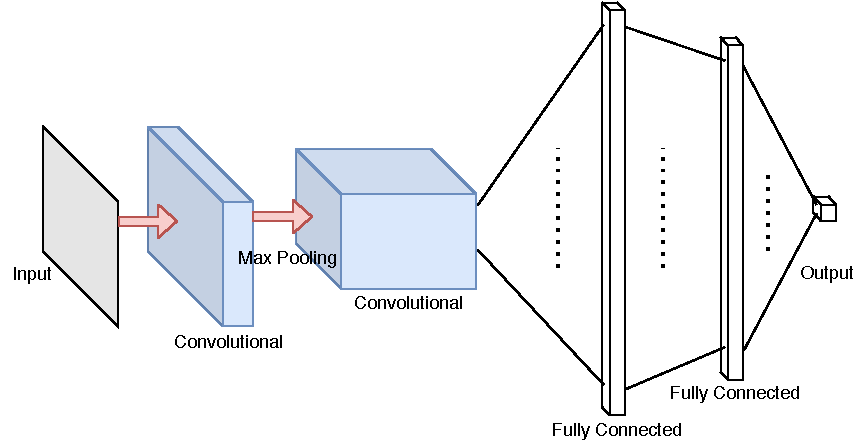
\includegraphics[width=1\textwidth]{IMPLEMENTATION_METHOD/model_SI-SO.pdf}
    \caption{Αρχιτεκτονική του μοντέλου μιας εισόδου---μιας εξόδου}
  \end{center}
\end{figure}
\section{Μοντέλο πολλαπλών εξόδων}
Μια δεύτερη υλοποίηση προτεινόμενου μοντέλου είναι η εξέλιξη του πρώτου μοντέλου σε ένα το οποίο θα εκτελεί πολλαπλές προβλέψεις ιδιοτήτων. Στην αρχιτεκτονική του μοντέλου υπάρχει η διαφορά πως διαθέτει πολλές εξόδους. Το σημείο στο οποίο δημιουργούνται οι πολλαπλές διεργασίες του μοντέλου είναι πριν από τα πλήρως συνδεδεμένα επίπεδα. Ένα μοντέλο το οποίο διαθέτει παραπάνω από μια εξόδους θεωρείται πως κατά την εκπαίδευση λαμβάνει πολυδιάστατες αναδράσεις σχετικά με τα σφάλματα πρόβλεψης του και ως αποτέλεσμα εκπαιδεύεται με πιο σφαιρικό τρόπο από ένα μοντέλο μιας εξόδου. Ωστόσο μια διαφορά σε σχέση με το μοντέλο μιας εξόδου είναι πως η επιλογή του βέλτιστου μοντέλου γίνεται με βάση το άθροισμα των σφαλμάτων επικύρωσης έτσι δεν είναι δεδομένο πως το μοντέλο θα έχει την βέλτιστη επίδοση για όλες τις ιδιότητες του σε αντίθεση με το δεύτερο στο οποίο για κάθε έξοδο γίνεται η εύρεση του βέλτιστου μοντέλου.

\begin{figure}[H]
  \begin{center}
    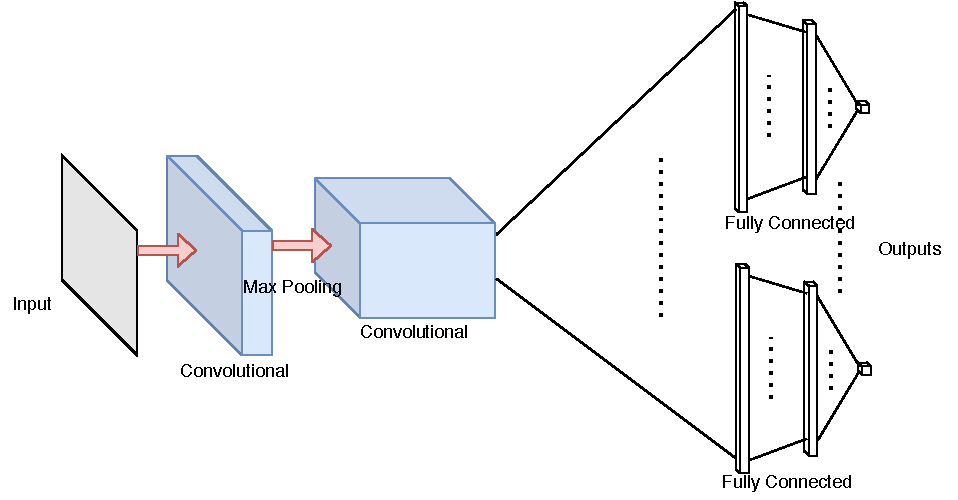
\includegraphics[width=1\textwidth]{IMPLEMENTATION_METHOD/model_SI-MO.pdf}
    \caption{Αρχιτεκτονική του μοντέλου μιας εισόδου---πολλαπλών εξόδων}
  \end{center}
\end{figure}

\section{Μοντέλο πολλαπλών εισόδων -- εξόδων}
Κατά την δοκιμή των πιθανών αρχιτεκτονικών που δοκιμάστηκαν έγινε η υπόθεση πως ένα μοντέλο το οποίο θα λαμβάνει πολλαπλά σπεκτρογράμματα μετασχηματισμών της εισόδου είναι πιθανό να έχει καλύτερη από ένα απλό μοντέλο μιας εισόδου. Η υπόθεση αυτή βασίζεται στην παρατήρηση πως για τις 2 διαφορετικές εισόδους της ανακλαστικότητας και της 1ης παραγώγου του μετασχηματισμού  \tl{Savitzky-Golay} της απορροφητικότητας το μοντέλο παρουσιάζει βέλτιστη επίδοση για διαφορετικές εξόδους σε κάθε είσοδο. Έτσι υποτίθεται πως η χρήση πολλαπλών εισόδων και εξόδων θα δύναται να παρέξει πληροφορία για την εξαγωγή των βέλτιστων προβλέψεων για όλες τις ιδιότητες εδάφους ενώ η εκπαίδευση του μοντέλου ευνοείται από τη χρήση πολλαπλών εξόδων.

\begin{figure}[H]
  \begin{center}
    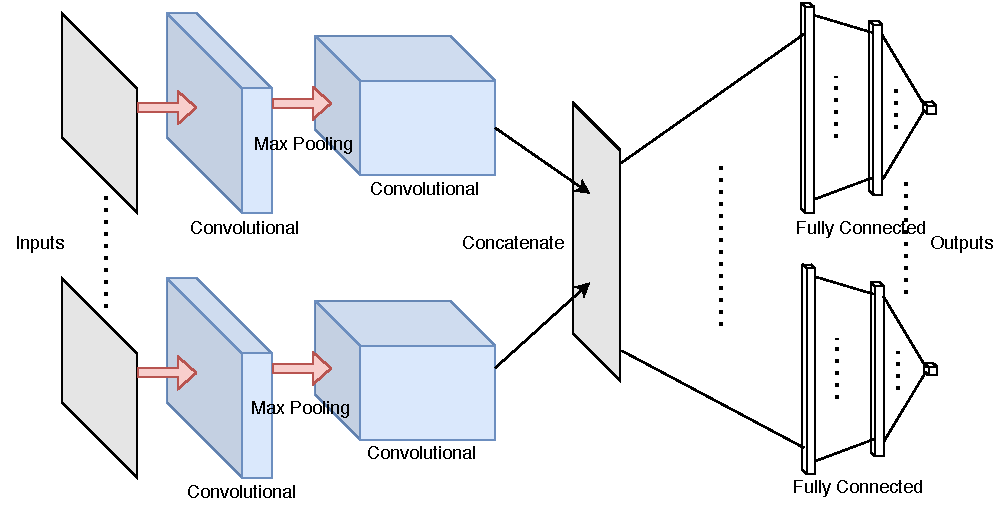
\includegraphics[width=1\textwidth]{IMPLEMENTATION_METHOD/model_MI-MO.pdf}
    \caption{Αρχιτεκτονική του μοντέλου πολλαπλών εισόδων---πολλαπλών εξόδων}
  \end{center}
\end{figure}

\section{Μοντέλο πολλαπλών εισόδων -- μιας εξόδου}
Στη συγκεκριμένη αρχιτεκτονική όπως και στην προηγούμενη υποενότητα γίνεται χρήση της πληροφορίας που παρέχεται από τις πολλαπλές εισόδους ενώ η εύρεση του βέλτιστου μοντέλου πραγματοποιείται με γνώμονα μια εδαφική ιδιότητα.
\begin{figure}[H]
  \begin{center}
    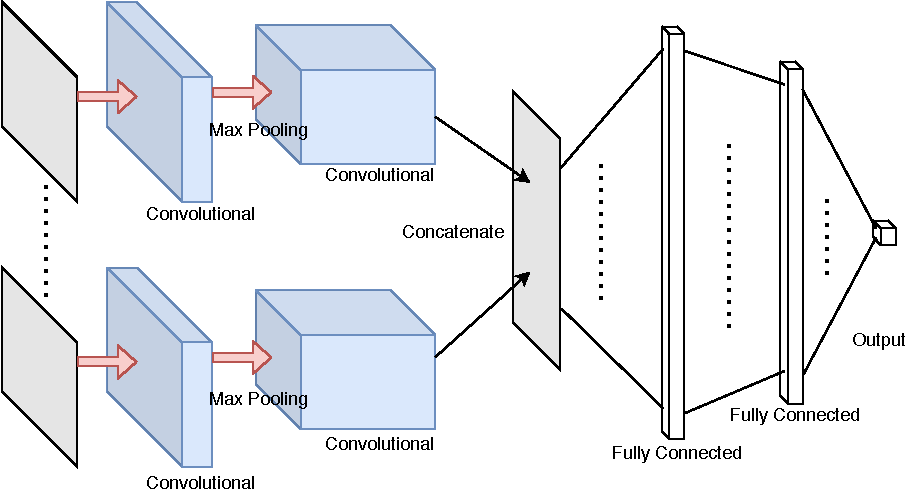
\includegraphics[width=1\textwidth]{IMPLEMENTATION_METHOD/model_MI-SO.pdf}
    \caption{Αρχιτεκτονική του μοντέλου πολλαπλών εισόδων---μιας εξόδου}
  \end{center}
\end{figure}
\section{Υλοποίηση εξαγωγής 1η παραγώγου μετασχηματισμού \tl{Savitzky Golay} απορροφητικότητας από ανακλαστικότητα}
Πρόλογος\\
Για εξαγωγή του συγκεκριμένου μετασχηματισμού αρχικά οι φασματικές υπογραφές ανακλασικότητας μετατρέπονται σε απορροφητικότητες. Η παραπάνω μετατροπή γίνεται με την εφαρμογή του παραπάνω τύπου στο φάσμα.
$$Absorbance=-log_{10}(Reflectance)$$

Η μορφή της φασματικής υπογραφής πριν και μετά την μετατροπή σε απορροφητικότητα φαίνεται στα σχήματα \ref{fig:abs_sg1_initial} και \ref{fig:abs_sg1_abs} αντίστοιχα.\\

Μετά τον μετασχηματισμό \tl{Savitzky-Golay} φαίνεται πως η φασματική υπογραφή έχει μεγάλες τιμές για τα αρχικά της δείγματα λόγω της μεγάλης κλίσης της φασματικής υπογραφής, κάτι που θα εισάγει μεγάλες τιμές στο δισδιάστατο συνελικτικό νευρωνικό δίκτυο για εκείνη την περιοχή του σήματος οι οποίες είναι πολύ μεγαλύτερες απο τις διακυμάνσεις σε όλη την υπόλοιπη έκταση του. Επίσης το εύρος τιμών της είναι πολύ μικρό σε σχέση με σχέση με τις τιμές της ανακλαστικότητας. Για την επίλυση των παραπάνω προβλημάτων αρχικά γίνεται κανονικοποίηση του φάσματος πολλαπλασιάζοντας την είσοδο με 333 και προσθέτοντας 0.5, έτσι το εύρος τιμών του μετασχηματισμένου σήματος είναι ίδιο με το αρχικό που έχει ανακλαστικότητα. Επίσης για την διόρθωση των ακραίων τιμών στα πρώτα δείγματα του σήματος εφαρμόζεται μια μάσκα για τον περιορισμό των τιμών στα πρώτα 100 δείγματα.//
Ο τύπος του μετασχηματισμού για τα 100 πρώτα δείγματα είναι ο εξής:
\[
    y[i]= 
\begin{cases}
    333\left(\frac{i}{100}\right)^{1,6}x[i]+0,5,& 0\leq x<100\\
    333 x[i]+0,5,              & 100\leq x<4200
\end{cases}
\]
Όπου $x[i]$ το δείγμα $i$ του φάσματος μετά τον μετασχηματισμό \tl{Savitzky-Golay} και $y[i]$ η τελική μορφή του σήματος.\\

Η μορφή της φασματικής υπογραφής όταν μετά τον μετασχηματισμό \tl{Savitzky-Golay} και τελικά μετά την κανονικοποίηση και την διόρθωση των αρχικών φαίνεται στα σχήματα \ref{fig:abs_sg1_transform_notches} και \ref{fig:abs_sg1_transform_fixed} αντίστοιχα.\\

\begin{figure}[htbp]
    \begin{subfigure}{0.5\textwidth}
        \includesvg[width=1\linewidth]{IMPLEMENTATION_METHOD/0_Initial}
        \caption{Αρχική μορφή φασματικής υπογραφής ανακλαστικότητας}
        \label{fig:abs_sg1_initial}
    \end{subfigure}
    \begin{subfigure}{0.5\textwidth}
        \includesvg[width=1\linewidth]{IMPLEMENTATION_METHOD/0_Abs}
        \caption{Μορφή φασματικής υπογραφής μετά τη μετατροπή σε απορροφητικότητα}
        \label{fig:abs_sg1_abs}
    \end{subfigure}
    \begin{subfigure}{0.5\textwidth}
        \includesvg[width=1\linewidth]{IMPLEMENTATION_METHOD/0_Abs_SG1}
        \caption{Φασματική υπογραφή μετά στον μετασχηματισμό \tl{}}
        \label{fig:abs_sg1_transform_notches}
    \end{subfigure}
    \begin{subfigure}{0.5\textwidth}
        \includesvg[width=1\linewidth]{IMPLEMENTATION_METHOD/0_Abs_SG1_Fixed}
        \caption{Μορφή φασματικής υπογραφής μετά τη μετατροπή σε απορροφητικότητα}
        \label{fig:abs_sg1_transform_fixed}
    \end{subfigure}
    \caption{Απεικόνιση φασματικής υπογραφής κατά τα στάδια της μετατροπής της σε μετασχηματισμό \tl{Savitzky-Golay} πρώτης παραγώγου}
\end{figure}


\section{Κανονικοποίηση δεδομένων εισόδου -- εξόδου}
Τα δεδομένα τα οποία θα εισαχθούν στο δισδιάστατο νευρωνικό δίκτυο θεωρείται πως είναι βέλτιστο να έχουν μια κατανομή η οποία θα οδηγεί σε παρόμοια εύρη τιμών, έτσι επιλέγεται η κανονικοποίηση με χρήση της μέσης τιμής και της διακύμανσης του εκάστοτε συνόλου. Με την τεχνική που χρησιμοποιείται τα δεδομένα έχουν μέση τιμή μηδέν και διακύμανση μονάδα.

\subsection{Κανονικοποίηση εισόδου}
Η είσοδος που προκύπτει από την μετασχηματισμό \tl{Fourier} βραχέως χρόνου είναι σε κλίμακα με μικρού εύρος τιμών και μικρής τάξης μεγέθους έτσι είναι απαραίτητη η χρήση της λογαριθμικής για την διάκριση των τιμών της εικόνας. Το αποτέλεσμα που προκύπτει μετά την λογαρίθμηση έχει σχετικά μεγάλες τιμές με εύρος $~[0,50]$, οπότε γίνεται κανονικοποίηση των τιμών στο διάστημα $[-1,1]$ όπως αναφέρεται παραπάνω ώστε να είναι σε μορφή εύχρηστη για την εισαγωγή τους στην είσοδο του δισδιάστατου συνελικτικού νευρωνικού δικτύου.
\subsection{Κανονικοποίηση εξόδου}
Ένας βασικός λόγος που η έξοδος κανονικοποιείται με μέση τιμή μηδέν και διακύμανση μονάδα είναι ώστε τα σφάλματα που προκύπτουν κατά την εκπαίδευση των μοντέλων πολλών εξόδων να είναι ισοδύναμα, ώστε να μην επιλέγεται κάποιο μοντέλο με βάση την βελτίωση της επίδοσης του σε μια συγκεκριμένη ιδιότητα.
\chapter{Πειράματα και Αποτελέσματα}
\label{ch:experiments_and_results}

\section{Υλικό διεξαγωγής πειραμάτων}
Για την εκτέλεση κώδικα με σκοπό την διεξαγωγή πειραμάτων απαιτείται η χρήση υπολογιστή ή μιας υπολογιστικής μονάδας. Στην υλοποίηση που απαιτείται για το αντικείμενο της συγκεκριμένης εργασίας ορισμένες διαδικασίες είναι αρκετά περίπλοκες και χρήζουν μεγάλης υπολογιστικής ισχύος. Οι διαδικασίες αυτές είναι η ανάγνωση και προ-επεξεργασία των δεδομένων, η εξαγωγή των σπεκτρογραμμάτων από τις φασματικές υπογραφές και το πιο σύνθετο η εκπαίδευση δισδιάστατων συνελικτικών νευρωνικών δικτύων.
Τα αποτελέσματα έχουν εξαχθεί αξιοποιώντας την Υπολογιστική Συστοιχία και τις παρεχόμενες υπηρεσίες υποστήριξης του Κέντρου Ηλεκτρονικής Διακυβέρνησης του Α.Π.Θ. \cite{hpcauth}, όπου η διαδικασία της εκπαίδευσης των μοντέλων επιταχύνεται με μια κάρτα γραφικών $NVIDIA~Tesla~P100$. Επίσης έγινε χρήση του προσωπικού υπολογιστή για κάποια από τα τελευταία πειράματα με τη χρήση κάρτας γραφικών $NVIDIA~RTX-2060$

\section{Τροποποίηση της αρχιτεκτονικής του μοντέλου}
Ένας από τους λόγους για τους οποίους η αρχιτεκτονική του μοντέλου των \tl{Padarian J. et al.} θεωρείται μη αποτελεσματική είναι ότι χρησιμοποιεί μεγάλο πλήθος επιπέδων. Πέρα από την επιρροή του αριθμού των επιπέδων στο μέγεθός των παραμέτρων του μοντέλου, η συγκεκριμένη αποτελεί μια παράμετρο η οποία δοκιμάστηκε σε διάφορες μορφές της μέσα στην αρχιτεκτονική του δισδιάστατου συνελικτικού νευρωνικού δικτύου όπως στο πλήθος των συνελικτικών επιπέδων που χρησιμοποιούνται, το πλήθος των πλήρων συνδεδεμένων επιπέδων ή η χρήση των επιπέδων συγκέντρωσης.\\

Για την σύγκριση των μοντέλων στο πειραματικό στάδιο χρησιμοποιήθηκαν τα μοντέλα μιας εισόδου με τη χρήση των σπεκτρογραμμάτων ανακλαστικότητας και πολλαπλών εξόδων για την πρόβλεψη των 6 βασικών ιδιοτήτων που εξετάζονται και στην δημοσίευση των \tl{Padarian et.al}, οι οποίες είναι σε συντομογραφίες οι \tl{OC, N, pH, Clay, Sand} και \tl{CEC}. Η επιλογή της παραπάνω μορφής μοντέλου επιλέχθηκε ώστε η διαδικασία εξαγωγής των αποτελεσμάτων να είναι συντομότερη ενώ τα αποτελέσματα να μπορούν να είναι βάσιμα.\\

Η προτεινόμενη αρχιτεκτονική των \tl{Padarian et al.} δίνεται στον Πίνακα~\ref{tab:padarian.network} με τα αποτελέσματα πρόβλεψης στο ανεξάρτητο σύνολο δεδομένων αξιολόγησης να δίνονται στα ραβδογράμματα του σχήματος ~\ref{fig:padarian.results}.

\begin{table}[!t]
    \centering
    \caption{Αρχιτεκτονική του προτεινόμενου μοντέλου}
    \label{tab:padarian.network}
    \ra{1.3}\selectlanguage{english}
    \begin{tabular}{@{}rrrrr@{}}\toprule
        Type&Kernel Size&Filters&Size&Activation\\
        \midrule
        Convolutional&$3 \times 3$&64&$51 \times 83$&ReLU\\
        Max-Pooling&$2 \times 2$&-&-&–\\
        Convolutional&$3 \times 3$&128&$25 \times 41$&ReLU\\
        Convolutional&$3 \times 3$&256&$25 \times 41$&ReLU\\
        Max-Pooling&$2 \times 2$&-&-&–\\
        Convolutional&$3 \times 3$&512&$12 \times 10$&ReLU\\
        Convolutional&$3 \times 3$&64&$12 \times 10$&ReLU\\
        Fully-connected&–&-&100&ReLU\\
        Fully-connected&–&-&1&Linear\\
        \addlinespace
        \textbf{Parameters}&–&\multicolumn{3}{c}{7,772,358}\\
        \bottomrule
    \end{tabular}\selectlanguage{greek}
\end{table}
\begin{figure}[!t]
    \selectlanguage{english}
    \begin{tikzpicture}
        \begin{axis}[
            ybar,
            width=19cm,
            height=11cm,
            bar width=21pt,
            enlargelimits=0.07,
            legend style={at={(0.8,0.95)},
              anchor=north,legend columns=1},
            ylabel={Coefficient of Determinanation $R^2$},
            symbolic x coords={OC, N, pH, Clay, Sand, CEC},
            xtick=data,
            nodes near coords,
            nodes near coords align={vertical},
            ]
                \addplot[fill=abs, draw=black] coordinates {(OC, 0.690) (N, 0.616) (pH, 0.843) (Clay, 0.611) (Sand, 0.543) (CEC, 0.606)};
                \addplot[fill=refl, draw=black] coordinates {(OC, 0.706) (N, 0.643) (pH, 0.808) (Clay, 0.646) (Sand, 0.547) (CEC, 0.606)};
        \legend{Suggested-Absorbances,Suggested-Reflectances}
        \end{axis}
    \end{tikzpicture}
    \selectlanguage{greek}
    \caption{Επιδόσεις του προτεινόμενου (\tl{Suggested}) μοντέλου για τις διαφορετικές εισόδους \tl{Absorbances-SG1} και \tl{Reflectances}}
    \label{fig:padarian.results}
\end{figure}
% \begin{table}[H]
%     \centering
%     \caption{Επίδοση του προτεινόμενου μοντέλου στο σετ δεδομένων αξιολόγησης (\tl{Test})}
%     \label{tab:padarian.results}
%     \ra{1.3}\selectlanguage{english}
%     \begin{tabular}{@{}rrrrrrr@{}}\toprule
%         Metric&OC&N&pH&Clay&Sand&CEC\\
%         \midrule
%         \textbf{Absorbances}&\multicolumn{6}{c}{}\\
%         RMSE&16.2137&1.0016&0.5227&8.0078&17.7052&6.4343\\
%         $R^2$&0.6906&0.6162&0.8437&0.6117&0.5432&0.6066\\
%         RPIQ&1.4123&1.3976&4.5718&2.2477&2.5416&1.8028\\
%         \addlinespace
%         \textbf{Reflectances}&\multicolumn{6}{c}{}\\
%         RMSE&15.7841&0.9658&0.5790&7.6366&17.6230&6.4378\\
%         $R^2$&0.7068&0.6432&0.8083&0.6468&0.5475&0.6062\\
%         RPIQ&1.4508&1.4495&4.1277&2.3570&2.5534&1.8018\\
%         \bottomrule
%     \end{tabular}\selectlanguage{greek}
% \end{table}

\subsection{Συνελικτικά επίπεδα}
Η αρχιτεκτονική του μοντέλου των \tl{Padarian et.al} θεωρείται πως περιλαμβάνει μεγάλο αριθμό συνελικτικών επιπέδων χωρίς αυτά να είναι απαραίτητα. Για την εξακρίβωση της παραπάνω υπόθεσης έγινε μια δοκιμή ενός μοντέλου το οποίο περιλαμβάνει 2 λιγότερα συνελικτικά επίπεδα και ένα λιγότερο επίπεδο συγκέντρωσης, επίσης προστέθηκε ένα ακόμη πλήρως συνδεδεμένο επίπεδο. Επίσης στην είσοδο του μοντέλου έχει εφαρμοστεί υποδειγματοληψία 1:8. Η αρχιτεκτονική καθώς και η επίδοση του μοντέλου φαίνεται στους παρακάτω πίνακες.

\begin{table}[!t]
    \centering
    \caption{Αρχιτεκτονική μοντέλου με μειωμένο αριθμό συνελικτικών επιπέδων}
    \ra{1.3}\selectlanguage{english}
    \begin{tabular}{@{}rrrrr@{}}\toprule
        Type&Kernel Size&Filters&Size&Activation\\
        \midrule
        Convolutional&$3 \times 3$&64&$9 \times 51$&ReLU\\
        Max-Pooling&$2 \times 2$&-&-&–\\
        Convolutional&$3 \times 3$&128&$4 \times 25$&ReLU\\
        Convolutional&$3 \times 3$&64&$4 \times 25$&ReLU\\
        Fully-connected&–&-&64&ReLU\\
        Fully-connected&–&-&32&ReLU\\
        Fully-connected&–&-&1&Linear\\
        \addlinespace
        \textbf{Parameters}&&\multicolumn{3}{c}{2,646,000}\\
        \bottomrule
    \end{tabular}\selectlanguage{greek}
\end{table}
\begin{figure}[!t]
    \selectlanguage{english}
    \begin{tikzpicture}
        \begin{axis}[
            ybar,
            width=19cm,
            height=11cm,
            bar width=15pt,
            enlargelimits=0.12,
            legend style={at={(0.8,0.95)},
              anchor=north,legend columns=1},
            ylabel={Coefficient of Determinanation $R^2$},
            symbolic x coords={OC, N, pH, Clay, Sand, CEC},
            xtick=data,
            nodes near coords,
            nodes near coords align={vertical},
            every node near coord/.append style={font=\footnotesize}
            ]
                \addplot[fill=abs, draw=black] coordinates {(OC, 0.690) (N, 0.616) (pH, 0.843) (Clay, 0.611) (Sand, 0.543) (CEC, 0.606)};
                \addplot[fill=refl, draw=black] coordinates {(OC, 0.706) (N, 0.643) (pH, 0.808) (Clay, 0.646) (Sand, 0.547) (CEC, 0.606)};
                \addplot[fill=abs1, draw=black] coordinates {(OC, 0.688) (N, 0.605) (pH, 0.859) (Clay, 0.627) (Sand, 0.566) (CEC, 0.598)};
                \addplot[fill=refl1, draw=black] coordinates {(OC, 0.709) (N, 0.626) (pH, 0.835) (Clay, 0.578) (Sand, 0.550) (CEC, 0.617)};
        \legend{Suggested-Abs-SG1,Suggested-Reflectances, Reduced-Abs-SG1, Reduced-Reflectances}
        \end{axis}
    \end{tikzpicture}
    \selectlanguage{greek}
    \caption{Επιδόσεις του μοντέλου με μειωμένα συνελικτικά επίπεδα (\tl{Reduced}) για τις διαφορετικές εισόδους \tl{Absorbances-SG1} και \tl{Reflectances} σε σύγκριση με το προτεινόμενο μοντέλο}
\end{figure}
% \begin{table}[H]
%     \centering
%     \caption{Επίδοση μοντέλου με μειωμένο αριθμό συνελικτικών επιπέδων στο σετ δεδομένων αξιολόγησης (\tl{Test})}
%     \ra{1.3}\selectlanguage{english}
%     \begin{tabular}{@{}rrrrrrr@{}}\toprule
%         Metric&OC&N&pH&Clay&Sand&CEC\\
%         \midrule
%         \textbf{Absorbances}&\multicolumn{6}{c}{}\\
%         RMSE&16.2720&1.0159&0.4953&7.8409&17.2600&6.5050\\
%         $R^2$&0.6884&0.6053&0.8598&0.6277&0.5660&0.5980\\
%         RPIQ&1.4073&1.3781&4.8258&2.2957&2.6072&1.7833\\
%         \midrule
%         \textbf{Reflectances}&\multicolumn{6}{c}{}\\
%         RMSE&15.7271&0.9880&0.5360&8.3438&17.5607&6.3457\\
%         $R^2$&0.7090&0.6266&0.8357&0.5784&0.5507&0.6174\\
%         RPIQ&1.4561&1.4170&4.4589&2.1573&2.5625&1.8280\\
%         \bottomrule
%     \end{tabular}\selectlanguage{greek}
% \end{table}

Με βάση τα αποτελέσματα του μοντέλου με μειωμένο αριθμό συνελικτικών επιπέδων προκύπτει το συμπέρασμα πως η χρήση της υποδειγματοληψίας και η μείωση των επιπέδων οδηγούν σε μια αρχιτεκτονική μοντέλου η οποία δύναται να έχει επιδόσεις αντίστοιχες με αυτές του προτεινόμενου μοντέλου.\\

\subsection{Πλήρως συνδεδεμένα επίπεδα}
Σε παρόμοια λογική με την προηγούμενη υποενότητα, για την αρχιτεκτονική του προτεινόμενου μοντέλου θεωρείται πως η χρήση ενός μόνο πλήρως συνδεδεμένου επιπέδου είναι ελλειπής, έτσι γίνεται μια δοκιμή ενός μοντέλου με αρχιτεκτονική που περιλαμβάνει 3 πλήρως συνδεδεμένα επίπεδα. Για την δοκιμή της συγκεκριμένης αρχιτεκτονικής αφαιρείται ένα ακόμη συνελικτικό επίπεδο σε σχέση με το τελευταίο μοντέλο, με σκοπό ο αριθμός των παραμέτρων να διατηρηθεί σε ένα λογικό πλαίσιο.

\begin{table}[H]
    \centering
    \caption{Αρχιτεκτονική μοντέλου με αυξημένο αριθμό πλήρως συνδεδεμένων επιπέδων}
    \label{tbl:arch-high-dense}
    \ra{1.3}\selectlanguage{english}
    \begin{tabular}{@{}rrrrr@{}}\toprule
        Type&Kernel Size&Filters&Size&Activation\\
        \midrule
        Convolutional&$3 \times 3$&64&$9 \times 51$&ReLU\\
        Max-Pooling&$2 \times 2$&-&-&–\\
        Convolutional&$3 \times 3$&128&$4 \times 25$&ReLU\\
        Fully-connected&–&-&128&ReLU\\
        Fully-connected&–&-&64&ReLU\\
        Fully-connected&–&-&32&ReLU\\
        Fully-connected&–&-&1&Linear\\
        \addlinespace
        \textbf{Parameters}&&\multicolumn{3}{c}{5,106,000}\\
        \bottomrule
    \end{tabular}\selectlanguage{greek}
\end{table}
\begin{figure}[H]
    \selectlanguage{english}
    \begin{tikzpicture}
        \begin{axis}[
            ybar,
            width=19cm,
            height=11cm,
            bar width=15pt,
            enlargelimits=0.12,
            legend style={at={(0.8,0.95)},
              anchor=north,legend columns=1},
            ylabel={Coefficient of Determinanation $R^2$},
            symbolic x coords={OC, N, pH, Clay, Sand, CEC},
            xtick=data,
            nodes near coords,
            nodes near coords align={vertical},
            every node near coord/.append style={font=\footnotesize}
            ]
                \addplot[fill=abs, draw=black] coordinates {(OC, 0.690) (N, 0.616) (pH, 0.843) (Clay, 0.611) (Sand, 0.543) (CEC, 0.606)};
                \addplot[fill=refl, draw=black] coordinates {(OC, 0.706) (N, 0.643) (pH, 0.808) (Clay, 0.646) (Sand, 0.547) (CEC, 0.606)};
                \addplot[fill=abs1, draw=black] coordinates {(OC, 0.680) (N, 0.559) (pH, 0.860) (Clay, 0.625) (Sand, 0.539) (CEC, 0.588)};
                \addplot[fill=refl1, draw=black] coordinates {(OC, 0.709) (N, 0.634) (pH, 0.840) (Clay, 0.633) (Sand, 0.556) (CEC, 0.615)};
        \legend{Suggested-Abs-SG1,Suggested-Reflectances, Reduced-Abs-SG1, Reduced-Reflectances}
        \end{axis}
    \end{tikzpicture}
    \selectlanguage{greek}
    \caption{Επιδόσεις του μοντέλου με μειωμένα συνελικτικά επίπεδα και αυξημένο αριθμό πλήρως συνδεδεμένων επιπέδων(\tl{Reduced}) για τις διαφορετικές εισόδους \tl{Absorbances-SG1} και \tl{Reflectances} σε σύγκριση με το προτεινόμενο μοντέλο για την μετρική $R^2$}
    \label{fig:perf-high-dense}
\end{figure}
% \begin{table}[H]
%     \centering
%     \caption{Επίδοση μοντέλου με αυξημένο αριθμό πλήρως συνδεδεμένων επιπέδων στο σετ δεδομένων αξιολόγησης (\tl{Test})}
%     \ra{1.3}\selectlanguage{english}
%     \begin{tabular}{@{}rrrrrrr@{}}\toprule
%         Metric&OC&N&pH&Clay&Sand&CEC\\
%         \midrule
%         \textbf{Absorbances}&\multicolumn{6}{c}{}\\
%         RMSE&16.4872&1.0732&0.4932&7.8613&17.7789&6.5797\\
%         $R^2$&0.6801&0.5595&0.8609&0.6258&0.5395&0.5887\\
%         RPIQ&1.3890&1.3045&4.8455&2.2897&2.5311&1.7630\\
%         \midrule
%         \textbf{Reflectances}&\multicolumn{6}{c}{}\\
%         RMSE&15.7040&0.9778&0.5278&7.7806&17.4388&6.3588\\
%         $R^2$&0.7098&0.6343&0.8407&0.6334&0.5569&0.6158\\
%         RPIQ&1.4582&1.4318&4.5280&2.3135&2.5805&1.8243\\
%         \bottomrule
%     \end{tabular}\selectlanguage{greek}
% \end{table}

Από τον πίνακα \ref{tbl:arch-high-dense} και το ραβδόγραμμα του σχήματος \ref{fig:perf-high-dense} φαίνεται πως η χρήση πλήρως συνδεδεμένων επιπέδων σε συνδυασμό με την μείωση των συνελικτικών επιπέδων στην αρχιτεκτονική του μοντέλου, εξάγει ισοδύναμα αποτελέσματα με το προτεινόμενο μοντέλο.

\subsection{Επιρροή χρήσης \tl{Max Pooling}}
Όπως αναφέρθηκε στην θεωρητική ανάλυση των δισδιάστατων νευρωνικών δικτύων, τα επίπεδα συγκέντρωσης είναι από τα βασικά της συγκεκριμένης κατηγορίας μοντέλων. Ωστόσο εξετάστηκε η επίδραση της μείωσης του αριθμού των επιπέδων συγκέντρωσης, καθώς σε ορισμένες αρχιτεκτονικές του δοκιμάστηκαν ο αριθμός των συνελικτικών επιπέδων φτάνει μέχρι και το ελάχιστο των 2 επιπέδων.

% \begin{table*}
%     \centering
%     \caption{Επίδοση μοντέλου χωρίς τη χρήση επιπέδου συγκέντρωσης}
%     \ra{1.3}\selectlanguage{english}
%     \begin{tabular}{@{}rrrrrrr@{}}\toprule
%         Metric&OC&N&pH&Clay&Sand&CEC\\
%         \midrule
%         \textbf{Absorbances}&\multicolumn{6}{c}{}\\
%         RMSE&15.9594&0.9958&0.4633&7.7620&17.3450&6.2407\\
%         $R^2$&0.7003&0.6207&0.8773&0.6352&0.5617&0.6300\\
%         RPIQ&1.4349&1.4059&5.1592&2.3190&2.5944&1.8588\\
%         \midrule
%         \textbf{Reflectances}&\multicolumn{6}{c}{}\\
%         RMSE&15.2674&0.9504&0.4820&7.1946&17.0409&6.1428\\
%         $R^2$&0.7257&0.6545&0.8672&0.6866&0.5769&0.6415\\
%         RPIQ&1.4999&1.4731&4.9590&2.5019&2.6407&1.8884\\
%         \bottomrule
%     \end{tabular}\selectlanguage{greek}
% \end{table*}
% \begin{table*}
%     \centering
%     \caption{Επίδοση μοντέλου με τη χρήση επιπέδου συγκέντρωσης στο σετ δεδομένων αξιολόγησης (\tl{Test})}
%     \ra{1.3}\selectlanguage{english}
%     \begin{tabular}{@{}rrrrrrr@{}}\toprule
%         Metric&OC&N&pH&Clay&Sand&CEC\\
%         \midrule
%         \textbf{Absorbances}&\multicolumn{6}{c}{}\\
%         RMSE&14.8639&0.9085&0.4440&7.1983&15.738&5.7918\\
%         $R^2$&0.7400&0.6843&0.8873&0.6862&0.639&0.6813\\
%         RPIQ&1.5406&1.5410&5.3830&2.5006&2.8593&2.0028\\
%         \midrule
%         \textbf{Reflectances}&\multicolumn{6}{c}{}\\
%         RMSE&14.2402&0.8777&0.4896&6.5591&15.8137&5.6772\\
%         $R^2$&0.7614&0.7054&0.8630&0.7395&0.6357&0.6938\\
%         RPIQ&1.6081&1.5951&4.8820&2.7443&2.8456&2.0433\\
%         \bottomrule
%     \end{tabular}\selectlanguage{greek}
% \end{table*}
\begin{figure}[H]
    \selectlanguage{english}
    \begin{tikzpicture}
        \begin{axis}[
            ybar,
            width=19cm,
            height=11cm,
            bar width=15pt,
            enlargelimits=0.12,
            legend style={at={(0.8,0.95)},
              anchor=north,legend columns=1},
            ylabel={Coefficient of Determinanation $R^2$},
            symbolic x coords={OC, N, pH, Clay, Sand, CEC},
            xtick=data,
            nodes near coords,
            nodes near coords align={vertical},
            every node near coord/.append style={font=\footnotesize}
            ]
                \addplot[fill=abs, draw=black] coordinates {(OC, 0.700)(N, 0.620)(pH, 0.877)(Clay, 0.635)(Sand, 0.561)(CEC, 0.630)};
                \addplot[fill=refl, draw=black] coordinates {(OC, 0.725)(N, 0.654)(pH, 0.867)(Clay, 0.686)(Sand, 0.576)(CEC, 0.641)};
                \addplot[fill=abs1, draw=black] coordinates {(OC, 0.740)(N, 0.684)(pH, 0.887)(Clay, 0.686)(Sand, 0.639)(CEC, 0.681)};
                \addplot[fill=refl1, draw=black] coordinates {(OC, 0.761)(N, 0.705)(pH, 0.863)(Clay, 0.739)(Sand, 0.635)(CEC, 0.693)};
        \legend{No-Pooling-Abs-SG1,No-Pooling-Reflectances, Pooling-Abs-SG1, Pooling-Reflectances}
        \end{axis}
    \end{tikzpicture}
    \selectlanguage{greek}
    \caption{Συγκρίσεις των επιδόσεων του μοντέλου με βάση την χρήση ή μη επιπέδων συγκέντρωσης μεγίστων (\tl{Max Pooling}) για τις διαφορετικές εισόδους \tl{Absorbances-SG1} και \tl{Reflectances} με βάση την μετρική του συντελεστή προσδιορισμού στο σετ αξιολόγησης}
\end{figure}

Σύμφωνα με τους παραπάνω πίνακες, φαίνεται πως η η αφαίρεση όλων των επιπέδων συγκέντρωσης έχει ως αποτέλεσμα την σημαντική μείωση της επίδοσης του μοντέλου. Επίσης είναι σημαντικό να αναφερθεί πως η συγκεκριμένη παράμετρος μπορεί να επηρεάσει σε μεγάλο βαθμό το συνολικό μέγεθος του μοντέλου, για παράδειγμα η αφαίρεση του επιπέδου συγκέντρωσης μεγίστων από το βέλτιστο μοντέλο πολλαπλών εισόδων και εξόδων έχει ως αποτέλεσμα η δομή του να έχει 12,746,886 παραμέτρους ενώ με ένα επίπεδο συγκέντρωσης μεγίστων έχει περίπου 2,891,910 παραμέτρους. Κατά την δοκιμή της χρήσης διαφόρων αριθμών επιπέδων συγκέντρωσης διαπιστώθηκε πως η βέλτιστη επίδοση του μοντέλου επιτυγχάνεται με χρήση ενός επιπέδου συγκέντρωσης μεγίστων.

\subsection{Επιρροή του λόγου οριζόντιας προς κατακόρυφης διάστασης}
Η παράμετρος που ορίζει τον λόγο τον διαστάσεων της εικόνας εισόδου κατά την μετατροπή της φασματικής υπογραφή σε σπεκτρόγραμμα, παρατηρήθηκε πως επηρεάζει καθοριστικά την επίδοση των υλοποιήσεων δισδιάστατων συνελικτικών νευρωνικών δικτύων.\\
Για την εύρεση της βέλτιστης τιμής της παραμέτρου \tl{V/H Ratio} χρησιμοποιήθηκε ένα μοντέλο πολλαπλών εισόδων και πολλαπλών εξόδων για την πρόβλεψη των περισσοτέρων ιδιοτήτων

\begin{figure}[H]
  \begin{center}
    \includesvg[width=1\textwidth]{RESULTS/Determ_v_h}
    \caption{Απόδοση του μοντέλου με βάση την μετρική $R^2$ συναρτήσει του λόγου κάθετης προς οριζόντιου διάστασης}
  \end{center}
\end{figure}

Όπως φαίνεται στο παραπάνω διάγραμμα, όταν η παράμετρος που ορίζει τον λόγο των διαστάσεων της εικόνας εισόδου, είναι στο εύρος τιμών 0.77 με 0.8 οι επιδόσεις του μοντέλου είναι κατά μέσο όρο μεγαλύτερες. Έτσι η τμή που επιλέχθηκε για τη συγκεκριμένη παράμετρο είναι το 0.8 καθώς παρουσιάζει την μέγιστη μέση επίδοση για τον συντελεστή προσδιορισμού όλων των εδαφικών ιδιοτήτων.

\subsection{Βέλτιστη αρχιτεκτονική μοντέλου}

Για τους συνδυασμούς των επιπέδων που χρησιμοποιούνται στην αρχιτεκτονική του μοντέλου έγιναν 10 πειράματα και η βέλτιστη αρχιτεκτονική του δισδιάστατου συνελικτικού νευρωνικού δικτύου που προέκυψε αποτελείται από τα επίπεδα του 

\begin{table}[H]
    \centering
    \caption{Αρχιτεκτονική του βέλτιστου μοντέλου}
    \label{fig:best_model}
    \ra{1.3}\selectlanguage{english}
    \begin{tabular}{@{}rrrrr@{}}\toprule
        Type&Kernel Size&Filters&Size&Activation\\
        \midrule
        Convolutional&$3 \times 3$&64&$9 \times 57$&ReLU\\
        Max-Pooling&$2 \times 2$&-&-&–\\
        Convolutional&$3 \times 3$&128&$4 \times 28$&ReLU\\
        Fully-connected&–&-&64&ReLU\\
        Fully-connected&–&-&32&ReLU\\
        Fully-connected&–&-&1&Linear\\
        \addlinespace
        \textbf{Parameters}&&\multicolumn{3}{c}{2,891,910}\\
        \bottomrule
    \end{tabular}\selectlanguage{greek}
\end{table}

\section{Επίδοση μοντέλων με χρήση μετασχηματισμών της εισόδου \tl{Abs-SG1 -- Reflectance spectrograms}}
\label{sec:refl-abs_sg1}
Η χρήση των σπεκτρογραμμάτων που προκύπτουν από την ανακλαστικότητα \tl{Reflectance} του εδάφους παρατηρήθηκε πως αποτελεί την καταλληλότερη είσοδο για την πρόβλεψη των περισσοτέρων ιδιοτήτων, η χρήση της συγκεκριμένης εισόδου  εφαρμόζεται και στην προτεινόμενη υλοποίηση. Ωστόσο έπειτα από δοκιμές χρήσης διαφόρων μετασχηματισμών της εισόδου στο μοντέλο και την εξαγωγή προβλέψεων του, παρατηρήθηκε πως η χρήση της 1ης παραγώγου του μετασχηματισμού \tl{Savitzky-Golay} έχει καλύτερες επιδόσεις σε ορισμένες ιδιότητες σε σχέση με τα σπεκτρογράμματα ανακλαστικότητας. Οι διαφορές φαίνονται αναλυτικά στα παρακάτω διαγράμματα.

\begin{figure}[H]
    \selectlanguage{english}
    \begin{tikzpicture}
        \begin{axis}[
            ybar,
            width=19cm,
            height=10cm,
            bar width=21pt,
            enlargelimits=0.07,
            legend style={at={(0.5,-0.1)},
              anchor=north,legend columns=-1},
            ylabel={Coefficient of Determinanation $R^2$},
            symbolic x coords={OC, CEC, Clay, Sand, Silt, pH, N, CaCO3, P, K},
            xtick=data,
            nodes near coords,
            nodes near coords align={vertical},
            ]
                \addplot[fill=abs, draw=black] coordinates {(OC, 0.755) (CEC, 0.708) (Clay, 0.713) (Sand, 0.666) (Silt, 0.615) (pH, 0.906) (N, 0.709) (CaCO3, 0.931) (P, 0.281) (K, 0.415)};
                \addplot[fill=refl, draw=black] coordinates {(OC, 0.768) (CEC, 0.726) (Clay, 0.766) (Sand, 0.768) (Silt, 0.631) (pH, 0.883) (N, 0.728) (CaCO3, 0.938) (P, 0.262) (K, 0.363)};
        \legend{Absorbances-SG1,Reflectances}
        \end{axis}
    \end{tikzpicture}
    \selectlanguage{greek}
    \caption{Σύγκριση επιδόσεων των μοντέλων μιας εισόδου---μιας εξόδου \tl{(SI--SO)} για τις διαφορετικές εισόδους \tl{Absorbances-SG1} και \tl{Reflectances}}
\end{figure}

\begin{figure}[H]
    \selectlanguage{english}
    \begin{tikzpicture}
        \begin{axis}[
            ybar,
            width=19cm,
            height=10cm,
            bar width=21pt,
            enlargelimits=0.07,
            legend style={at={(0.5,-0.1)},
              anchor=north,legend columns=-1},
            ylabel={Coefficient of Determinanation $R^2$},
            symbolic x coords={OC, CEC, Clay, Sand, Silt, pH, N, CaCO3, P, K},
            xtick=data,
            nodes near coords,
            nodes near coords align={vertical},
            ]
                \addplot[fill=abs, draw=black] coordinates {(OC, 0.751) (CEC, 0.708) (Clay, 0.714) (Sand, 0.663) (Silt, 0.559) (pH, 0.901) (N,0.716) (CaCO3, 0.931) (P, 0.284) (K, 0.431)};
                \addplot[fill=refl, draw=black] coordinates {(OC, 0.775) (CEC, 0.722) (Clay, 0.766) (Sand, 0.672) (Silt, 0.577) (pH, 0.877) (N,0.730) (CaCO3, 0.937) (P, 0.270) (K, 0.376)};
        \legend{Absorbances-SG1,Reflectances}
        \end{axis}
    \end{tikzpicture}
    \selectlanguage{greek}
    \caption{Σύγκριση επιδόσεων των μοντέλων μιας εισόδου---πολλαπλών εξόδων \tl{(SI--MO)} για τις διαφορετικές εισόδους \tl{Absorbances-SG1} και \tl{Reflectances}}
\end{figure}

Όπως προκύπτει και από τους 2 τύπους μοντέλων μιας εισόδου με βάση τα παραπάνω διαγράμματα των σχημάτων, οι προβλέψεις των μοντέλων με είσοδο τα σπεκτρογράμματα του μετασχηματισμού \tl{Savitzky-Golay} πρώτης παραγώγου της απορροφητικότητας έχουν καλύτερες επιδόσεις για τις ιδιότητες του \tl{pH} στο νερό, της περιεκτικότητας καλίου και φωσφόρου, ενώ ελαφρώς χειρότερη επίδοση από το μοντέλο που χρησιμοποιεί τα σπεκτρογράμματα από ανακλαστικότητα για τις υπόλοιπες ιδιότητες \tl{Organic Carbon, Nitrogen, Cation Exchange Capacity, Clay, Sand}.

\section{Επίδοση μοντέλου με χρήση πολλαπλών εισόδων}
Έπειτα από την δοκιμή της επίδοσης των 2 ξεχωριστών εισόδων έγινε μια απόπειρα για την χρήση και των 2 εισόδων σε ένα μοντέλο με σκοπό την επίτευξη καλύτερων επιδόσεων. Το αποτέλεσμα πράγματα δείχνει μια βελτίωση της επίδοσης του μοντέλου πολλαπλών εισόδων, με την τήρηση του βέλτιστου αποτελέσματος για την κάθε είσοδο, ενώ ταυτόχρονα παρατηρήθηκε μια συνολική βελτίωση της επίδοσης του νευρωνικού δικτύου.

\section{Επίδοση μοντέλων πολλαπλών εξόδων -- μιας εξόδου}
Η απόπειρα πρόβλεψης πολλαπλών ιδιοτήτων με τη χρήση ενός μοντέλου, απαιτεί μια πολυπλοκότερη διαδικασία εκπαίδευσης λόγω του μεγέθους του νέου μοντέλου. Το αποτέλεσμα ωστόσο είναι ικανοποιητικό. Παρόλο που παρατηρείται μια ελαφρώς χειρότερη επίδοση για όλες τις εξόδους, οι προβλέψεις του μοντέλου είναι κοντά σε αυτές των μοντέλων πρόβλεψης μιας ιδιότητας εδάφους, πράγμα που δείχνει πως η διαδικασία εκπαίδευσης ενός ξεχωριστού μοντέλου για κάθε ιδιότητα είναι σπάταλη. Αυτό διαπιστώνεται με την διαφορά στον χρόνο εκπαίδευσης των 2 ειδών μοντέλων, αλλά λόγω την πρακτική της εξαγωγής αποτελεσμάτων, επειδή χρειάζονται τόσα διαφορετικά μοντέλα όσες και οι ιδιότητες που προβλέπονται. Ωστόσο το πλήθος των παραμέτρων είναι ανάλογο του αριθμού των εξόδων του μοντέλου, σε σχέση με ένα μοντέλο μιας εξόδου.

Κάτι που πρέπει να αναφερθεί είναι πως η εξαγωγή προβλέψεων για την ιδιότητα της περιεκτικότητας των υλικών υφής σε ιλύ \tl{Silt}, για τα μοντέλα πολλαπλών εξόδων η συγκεκριμένη έξοδος αφαιρέθηκε από τα μοντέλα καθώς παρατηρήθηκε η μείωση της μέσης επίδοσης του μοντέλου για όλες τις υπόλοιπες ιδιότητες. Έτσι για την πρόβλεψη αυτής της εδαφικής ιδιότητας χρησιμοποιήθηκαν οι προβλέψεις του μοντέλου για τις ιδιότητες της άμμου \tl{Sand} και του άργιλου \tl{Clay}, με την εφαρμογή του τύπου $Silt=100-Sand-Clay$, ενώ για τα μοντέλα μιας εξόδου εκπαίδευτηκε κανονικά μοντέλο και για αυτή την ιδιότητα.

\section{Διαγράμματα σύγκρισης μοντέλων με την προτεινόμενη υλοποίηση}

Στην συγκεκριμένη υποενότητα θα παρουσιαστούν οι διάφορες πιθανές υλοποιήσεις του βέλτιστου μοντέλου σε σύγκριση με τις προτεινόμενες υλοποιήσεις. Τα μοντέλα που συγκρίνονται είναι τα \tl{Suggested SISO} και \tl{SIMO} δηλαδή τα προτεινόμενα μοντέλα στην μορφή μιας εισόδου και μιας ή πολλαπλών εξόδων για κάθε εδαφική ιδιότητα τα οποία έχουν δοκιμαστεί σύμφωνα με τις παραμέτρους της μεθοδολογίας των \tl{Padarian et.al}. Οι παράμετροι είναι, η χρήση 20 εποχών για την εκπαίδευση και της παρτίδας κανονικοποίησης μεγέθους 10 ενώ χρησιμοποιήθηκε ο βελτιστοποιητής \tl{Adam}. Τα μοντέλα τα οποία παρουσιάζονται ως βέλτιστα σύμφωνα με την μεθοδολογία της παρούσας διπλωματικής εργασίας είναι τα \tl{Reduced SISO, SIMO, MIMO} και \tl{MISO} τα οποία προκύπτουν από όλους τα πιθανούς συνδυασμούς πλήθους εισόδων και εξόδων. Η αρχιτεκτονική του είναι της μορφής του πίνακα \ref{fig:best_model}, ενώ οι παράμετροι τους είναι, 100 εποχές για την εκπαίδευση των μοντέλων μιας εισόδου η 300 εποχές για τα μοντέλα πολλαπλών εξόδων, μέγεθος κανονικοποίησης παρτίδας 48 και χρήση του βελτιστοποιητή \tl{Nadam}.\\

Για τα μοντέλα μιας εισόδου χρησιμοποιήθηκε μόνο η είσοδος των σπεκτρογραμμάτων ανακλαστικότητας ώστε να υπάρχει μια κοινή βάση σύγκρισης, αλλά και για απλούστευση της διαδικασίας με την αποφυγή της επιλογής των μοντέλων, με χρήση διαφορετικής εισόδου κάθε φορά ανά ιδιότητα όπως θα προέκυπτε ιδανικά από τα συμπεράσματα της υποενότητας \ref{sec:refl-abs_sg1}. Στις εξόδους των μοντέλων προβλέπονται όλες οι εδαφικές ιδιότητες που αναφέρθηκαν στην υποενότητα \ref{sec:props-spectrograms} του κεφαλαίου \ref{ch:lucas_soil}.\\

Στα παρακάτω διαγράμματα φαίνονται τα θηκογράμματα του απόλυτου σφάλματος των μοντέλων προς σύγκριση. Σε κάθε θηκόγραμμα έχουν αγνοηθεί ορισμένες εξωκείμενες τιμές με σκοπό την καθαρή απεικόνιση του τυπικού εύρους των σφαλμάτων πρόβλεψης.

\begin{figure}[H]
    \begin{subfigure}{0.5\textwidth}
        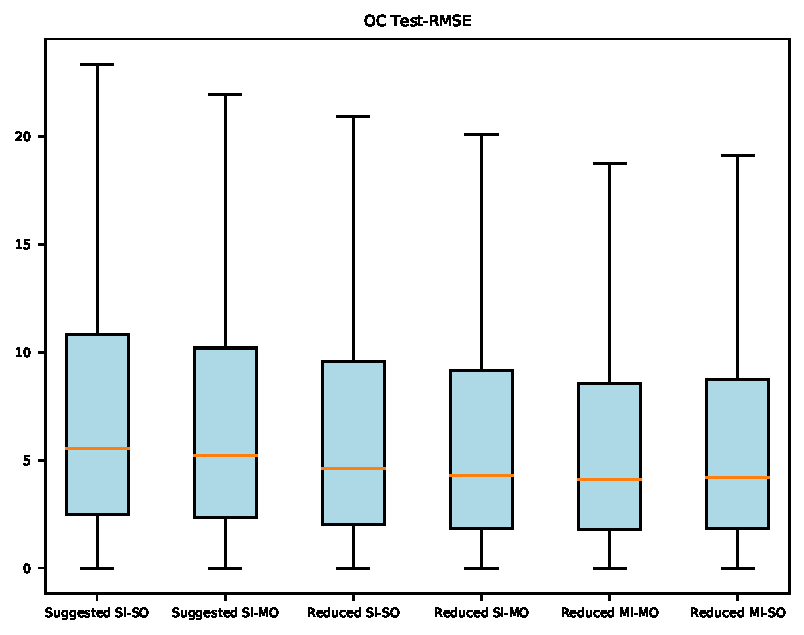
\includegraphics[width=1\linewidth]{RESULTS/BOXPLOTS/OC.pdf}
        \caption{Σύγκριση μοντέλων για την ιδιότητα του οργανικού άνθρακα}
        \label{fig:OC_boxplot}
    \end{subfigure}
    \begin{subfigure}{0.5\textwidth}
        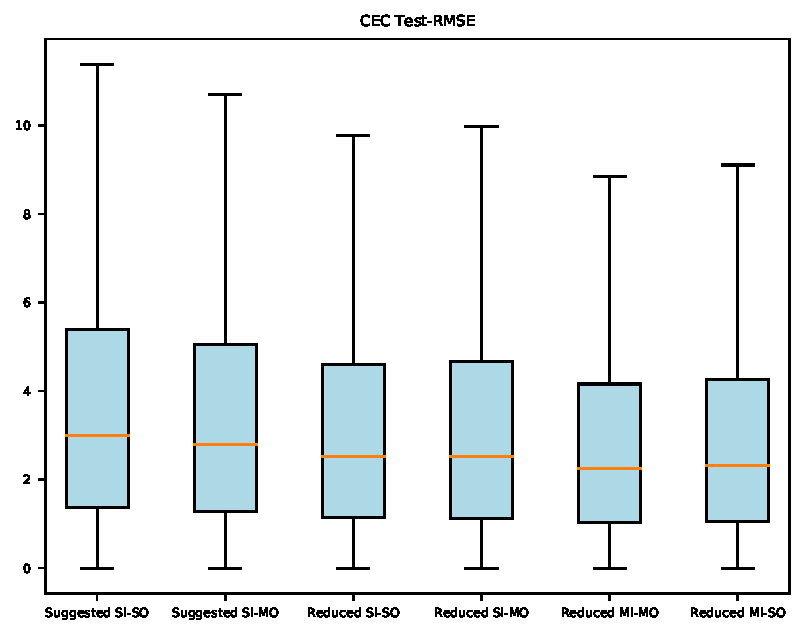
\includegraphics[width=1\linewidth]{RESULTS/BOXPLOTS/CEC.pdf}
        \caption{Σύγκριση μοντέλων για την ιδιότητα της ικανότητας ανταλλαγής κατιόντων}
        \label{fig:CEC_boxplot}
    \end{subfigure}
    \caption{Θηκογράμματα απόλυτου σφάλματος για τις ιδιότητες \tl{OC} και \tl{CEC}}
    \label{fig:boxpl-OC-CEC}
\end{figure}
\begin{figure}[H]
    \begin{subfigure}{0.5\textwidth}
        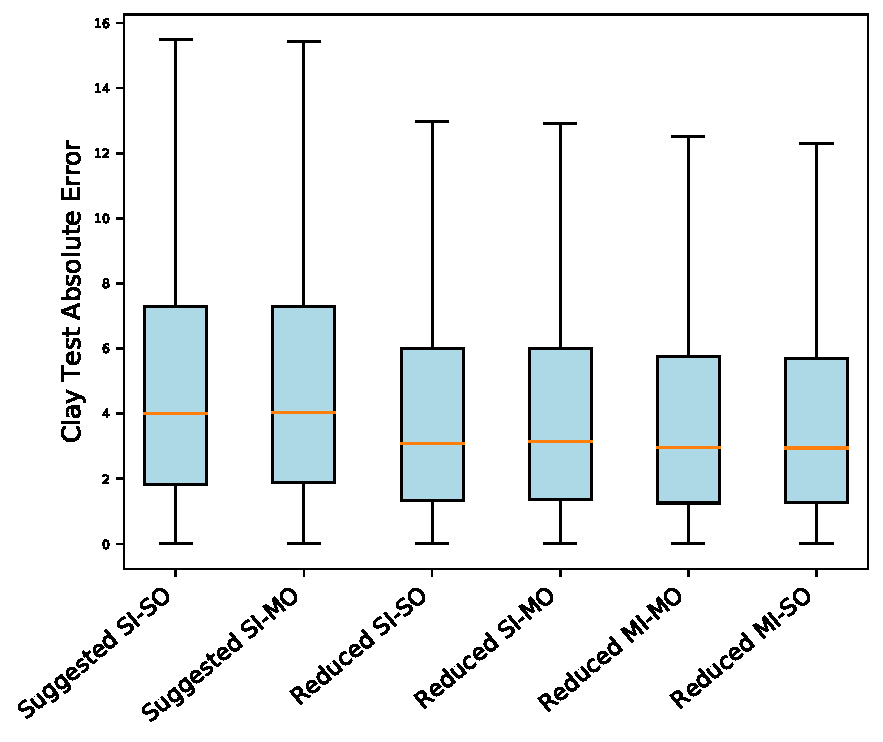
\includegraphics[width=1\linewidth]{RESULTS/BOXPLOTS/Clay.pdf}
        \caption{Σύγκριση μοντέλων για την ιδιότητα της περιεκτικότητας σε άργιλο}
        \label{fig:Clay_boxplot}
    \end{subfigure}
    \begin{subfigure}{0.5\textwidth}
        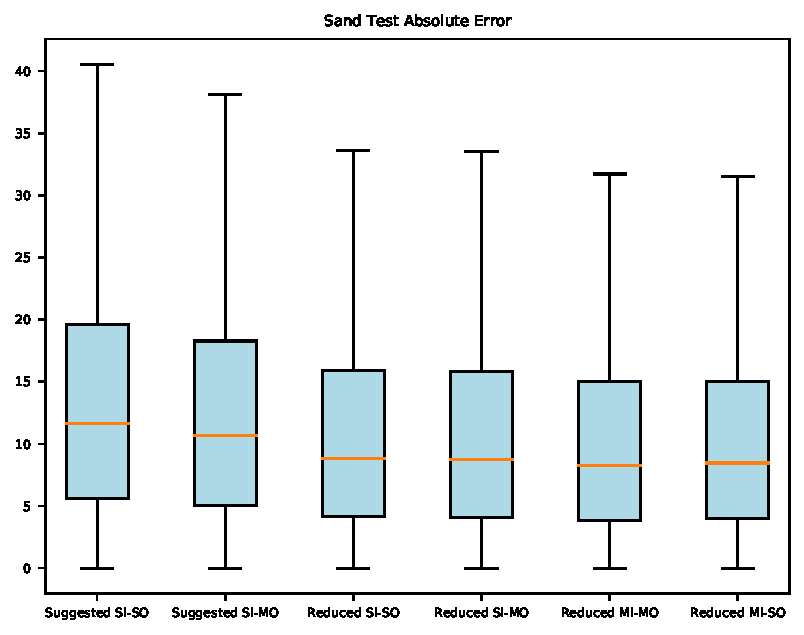
\includegraphics[width=1\linewidth]{RESULTS/BOXPLOTS/Sand.pdf}
        \caption{Σύγκριση μοντέλων για την ιδιότητα της περιεκτικότητας σε άμμο}
        \label{fig:Sand_boxplot}
    \end{subfigure}
    \caption{Θηκογράμματα απόλυτου σφάλματος για τις ιδιότητες \tl{Clay} και \tl{Sand}}
    \label{fig:boxpl-Clay-Sand}
\end{figure}
\begin{figure}[H]
    \begin{subfigure}{0.5\textwidth}
        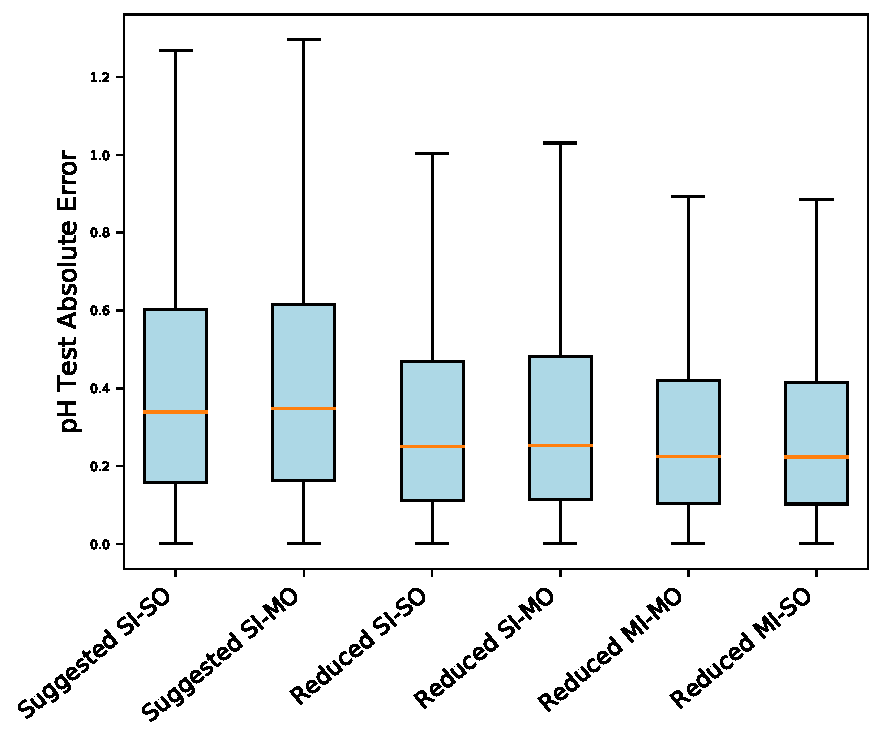
\includegraphics[width=1\linewidth]{RESULTS/BOXPLOTS/pH.pdf}
        \caption{Σύγκριση μοντέλων για την ιδιότητα του \tl{pH} στο νερό του εδάφους}
        \label{fig:pH_boxplot}
    \end{subfigure}
    \begin{subfigure}{0.5\textwidth}
        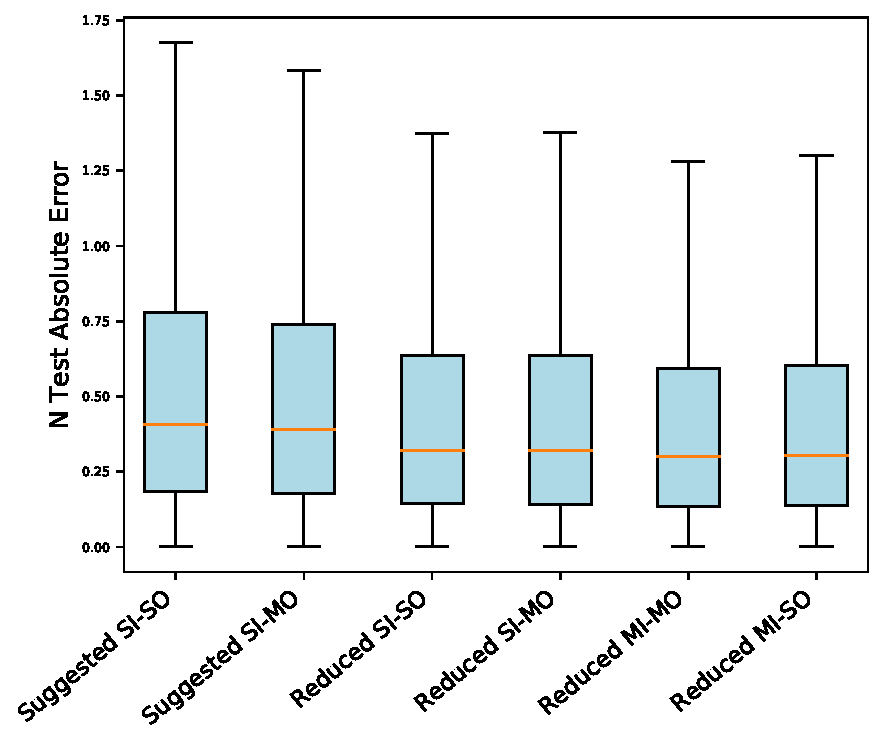
\includegraphics[width=1\linewidth]{RESULTS/BOXPLOTS/N.pdf}
        \caption{Σύγκριση μοντέλων για την ιδιότητα της περιεκτικότητας του αζώτου στο έδαφος}
        \label{fig:N_boxplot}
    \end{subfigure}
    \caption{Θηκογράμματα απόλυτου σφάλματος για τις ιδιότητες \tl{pH} και \tl{N}}
    \label{fig:boxpl-pH-N}
\end{figure}
\begin{figure}[H]
    \begin{subfigure}{0.5\textwidth}
        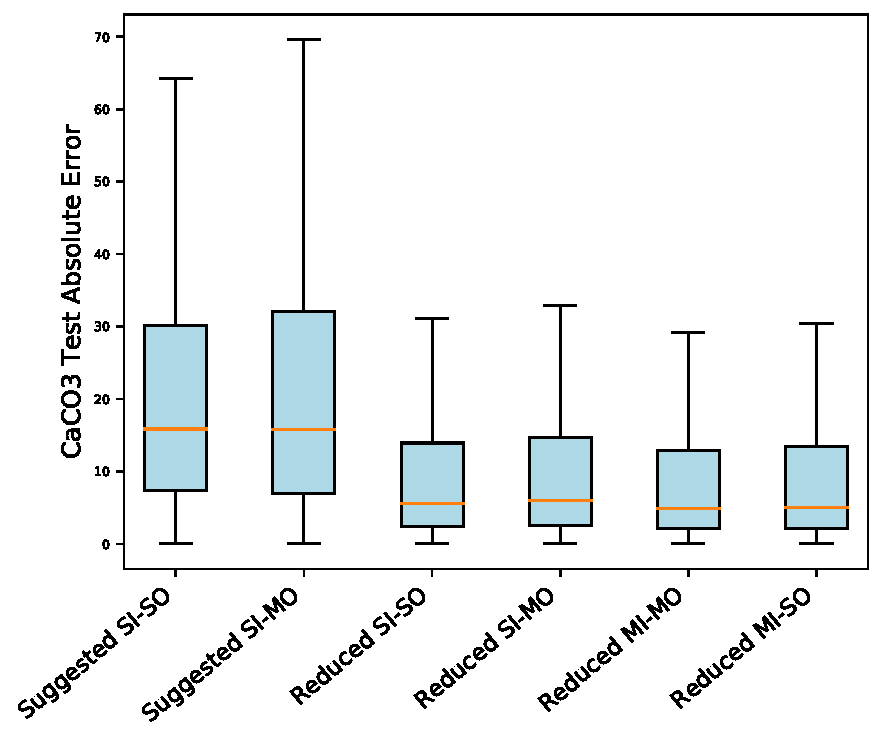
\includegraphics[width=1\linewidth]{RESULTS/BOXPLOTS/CaCO3.pdf}
        \caption{Σύγκριση μοντέλων για την ιδιότητα της περιεκτικότητας ανθρακικού ασβεστίου στο έδαφος}
        \label{fig:CaCO3_boxplot}
    \end{subfigure}
    \begin{subfigure}{0.5\textwidth}
        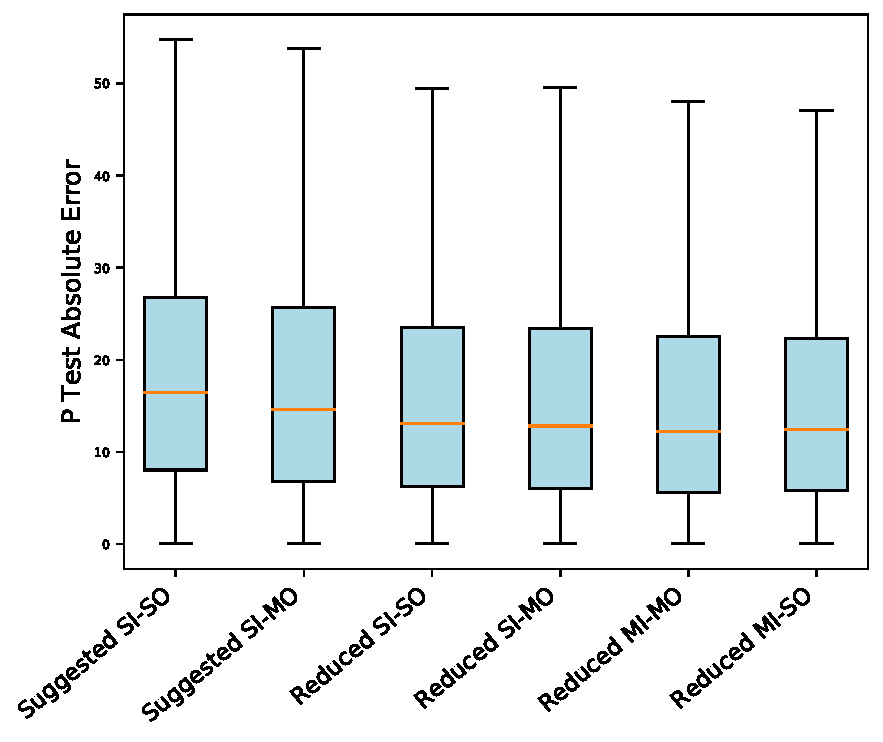
\includegraphics[width=1\linewidth]{RESULTS/BOXPLOTS/P.pdf}
        \caption{Σύγκριση μοντέλων για την ιδιότητα της περιεκτικότητας του φωσφόρου στο έδαφος}
        \label{fig:P_boxplot}
    \end{subfigure}
    \caption{Θηκογράμματα απόλυτου σφάλματος για τις ιδιότητες \tl{CaCO3} και \tl{P}}
    \label{fig:boxpl-CaCO3-P}
\end{figure}
\begin{figure}[H]
    \begin{subfigure}{0.5\textwidth}
        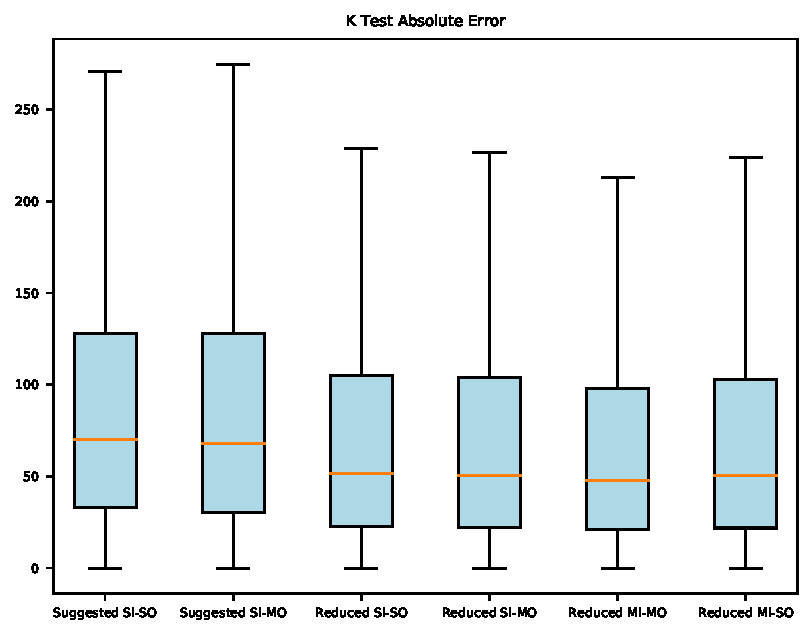
\includegraphics[width=1\linewidth]{RESULTS/BOXPLOTS/K.pdf}
        \caption{Σύγκριση μοντέλων για την ιδιότητα της περιεκτικότητας του καλίου στο έδαφος}
        \label{fig:K_boxplot}
    \end{subfigure}
    \begin{subfigure}{0.5\textwidth}
        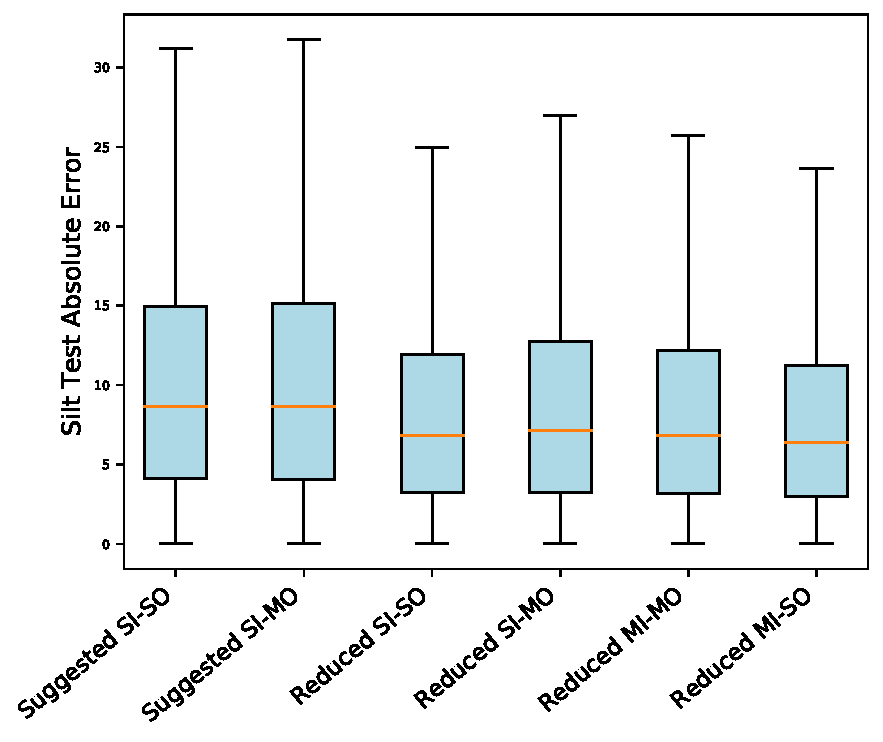
\includegraphics[width=1\linewidth]{RESULTS/BOXPLOTS/Silt.pdf}
        \caption{Σύγκριση μοντέλων για την ιδιότητα της περιεκτικότητας του εδάφους σε ιλύ}
        \label{fig:Silt_boxplot}
    \end{subfigure}
    \caption{Θηκογράμματα απόλυτου σφάλματος για τις ιδιότητες \tl{K} και \tl{Silt}}
    \label{fig:boxpl-K-Silt}
\end{figure}

Στα θηκογράμματα των σχημάτων \ref{fig:boxpl-OC-CEC} με \ref{fig:boxpl-K-Silt} φαίνεται πως η επίδοση των βέλτιστων μοντέλων είναι αισθητά καλύτερη από αυτή των προτεινόμενων κάτι που εξακριβώνεται από την θέση της διαμέσου $Q_{50}$ αλλά και της μορφής του διαστήματος μεταξύ του 3ου $Q_{75}$ τεταρτημορίου και του μέγιστου σφάλματος. Ανάμεσα στα μοντέλα της βέλτιστης αρχιτεκτονικής φαίνεται πως η χρήση πολλαπλών εισόδων έχει αυξημένες επιδόσεις σε σχέση με αυτά της μονής εισόδου σπεκτρογράμματος ανακλαστικότητας για αρκετές από τις ιδιότητες.

\begin{figure}[H]
    \begin{subfigure}{0.5\textwidth}
        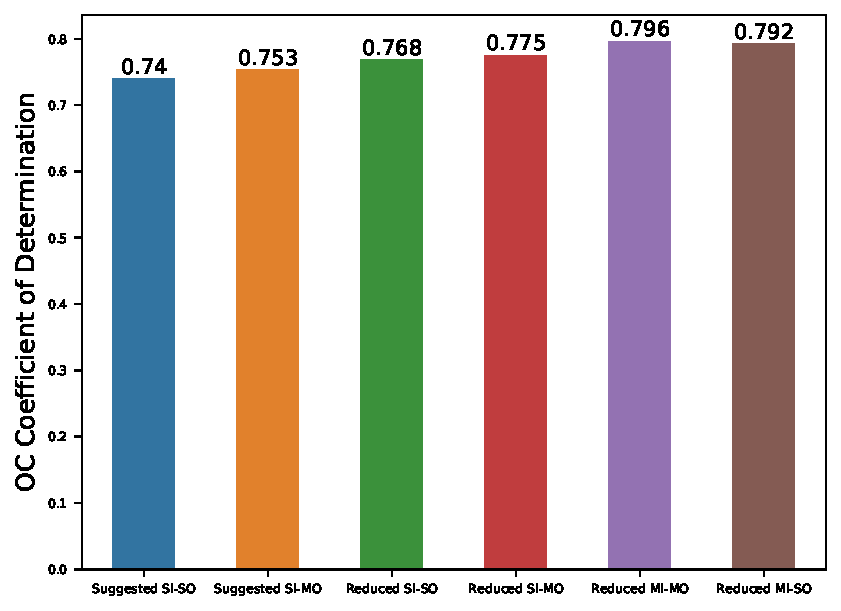
\includegraphics[width=1\linewidth]{RESULTS/BARPLOTS/test_OC_determ.pdf}
        \caption{Σύγκριση μοντέλων για την ιδιότητα του οργανικού άνθρακα}
        \label{fig:OC_determ}
    \end{subfigure}
    \begin{subfigure}{0.5\textwidth}
        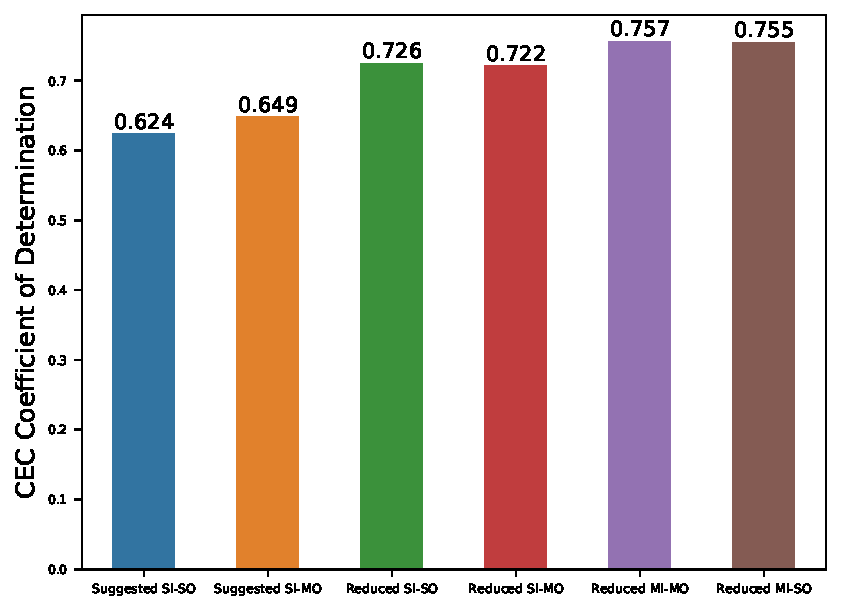
\includegraphics[width=1\linewidth]{RESULTS/BARPLOTS/test_CEC_determ.pdf}
        \caption{Σύγκριση μοντέλων για την ιδιότητα της ικανότητας ανταλλαγής κατιόντων}
        \label{fig:CEC_determ}
    \end{subfigure}
    \caption{Ραβδογράμματα συντελεστή προσδιορισμού για τις ιδιότητες \tl{OC} και \tl{CEC}}
    \label{fig:barpl-OC-CEC}
\end{figure}
\begin{figure}[H]
    \begin{subfigure}{0.5\textwidth}
        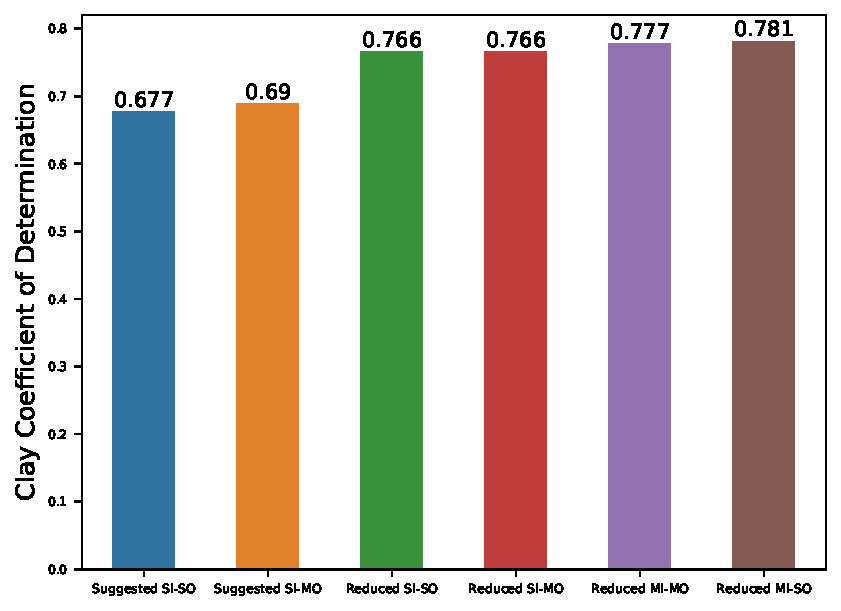
\includegraphics[width=1\linewidth]{RESULTS/BARPLOTS/test_Clay_determ.pdf}
        \caption{Σύγκριση μοντέλων για την ιδιότητα της περιεκτικότητας σε άργιλο}
        \label{fig:Clay_determ}
    \end{subfigure}
    \begin{subfigure}{0.5\textwidth}
        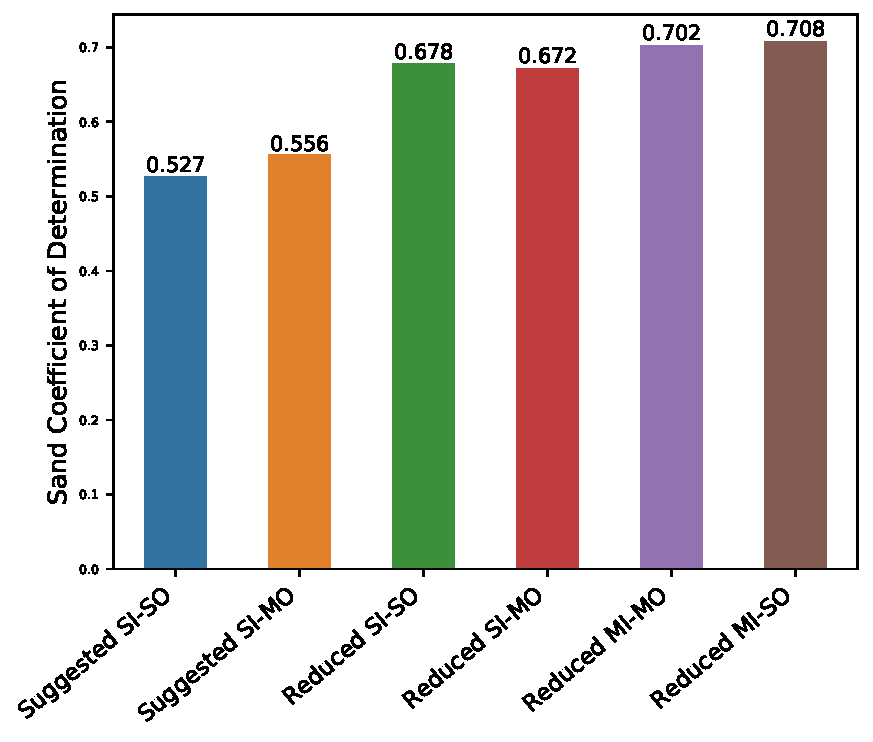
\includegraphics[width=1\linewidth]{RESULTS/BARPLOTS/test_Sand_determ.pdf}
        \caption{Σύγκριση μοντέλων για την ιδιότητα της περιεκτικότητας σε άμμο}
        \label{fig:Sand_determ}
    \end{subfigure}
    \caption{Ραβδογράμματα συντελεστή προσδιορισμού για τις ιδιότητες \tl{Clay} και \tl{Sand}}
    \label{fig:barpl-Clay-Sand}
\end{figure}
\begin{figure}[H]
    \begin{subfigure}{0.5\textwidth}
        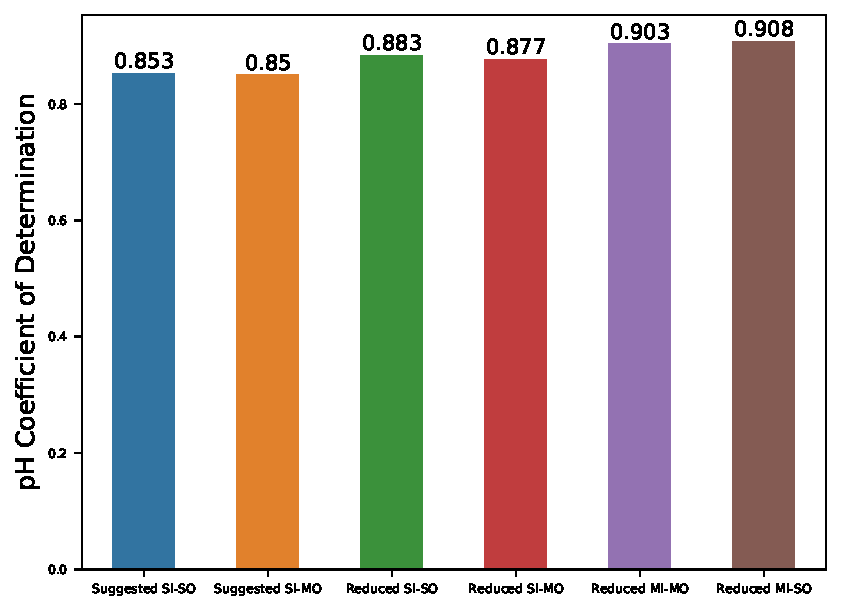
\includegraphics[width=1\linewidth]{RESULTS/BARPLOTS/test_pH_determ.pdf}
        \caption{Σύγκριση μοντέλων για την ιδιότητα του \tl{pH} στο νερό του εδάφους}
        \label{fig:pH_determ}
    \end{subfigure}
    \begin{subfigure}{0.5\textwidth}
        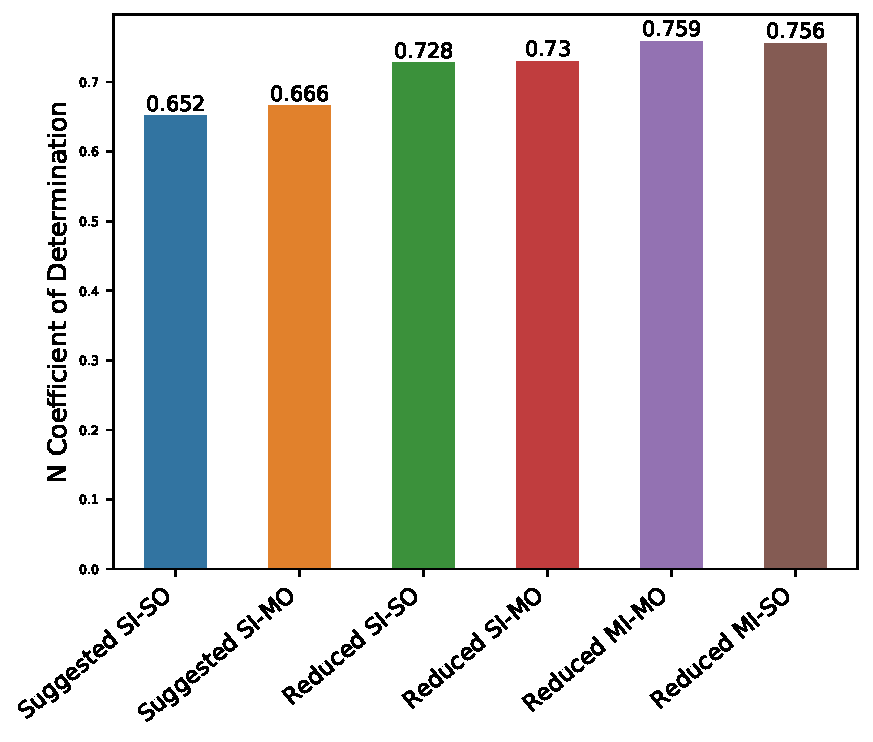
\includegraphics[width=1\linewidth]{RESULTS/BARPLOTS/test_N_determ.pdf}
        \caption{Σύγκριση μοντέλων για την ιδιότητα της περιεκτικότητας του αζώτου στο έδαφος}
        \label{fig:N_determ}
    \end{subfigure}
    \caption{Ραβδογράμματα συντελεστή προσδιορισμού για τις ιδιότητες \tl{pH} και \tl{N}}
    \label{fig:barpl-pH-N}
\end{figure}
\begin{figure}[H]
    \begin{subfigure}{0.5\textwidth}
        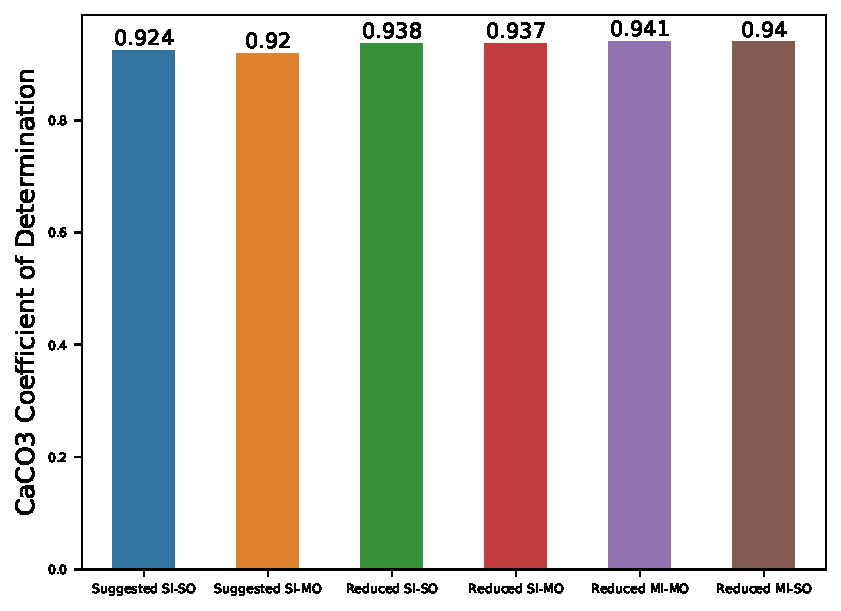
\includegraphics[width=1\linewidth]{RESULTS/BARPLOTS/test_CaCO3_determ.pdf}
        \caption{Σύγκριση μοντέλων για την ιδιότητα της περιεκτικότητας ανθρακικού ασβεστίου στο έδαφος}
        \label{fig:CaCO3_determ}
    \end{subfigure}
    \begin{subfigure}{0.5\textwidth}
        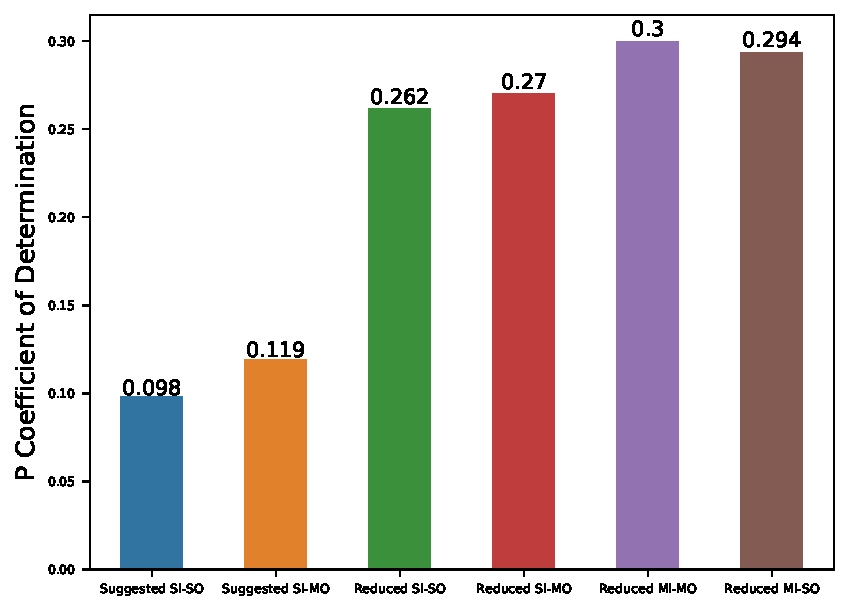
\includegraphics[width=1\linewidth]{RESULTS/BARPLOTS/test_P_determ.pdf}
        \caption{Σύγκριση μοντέλων για την ιδιότητα της περιεκτικότητας του φωσφόρου στο έδαφος}
        \label{fig:P_determ}
    \end{subfigure}
    \caption{Ραβδογράμματα συντελεστή προσδιορισμού για τις ιδιότητες \tl{CaCO3} και \tl{P}}
    \label{fig:barpl-CacCO3-Pc}
\end{figure}
\begin{figure}[H]
    \begin{subfigure}{0.5\textwidth}
        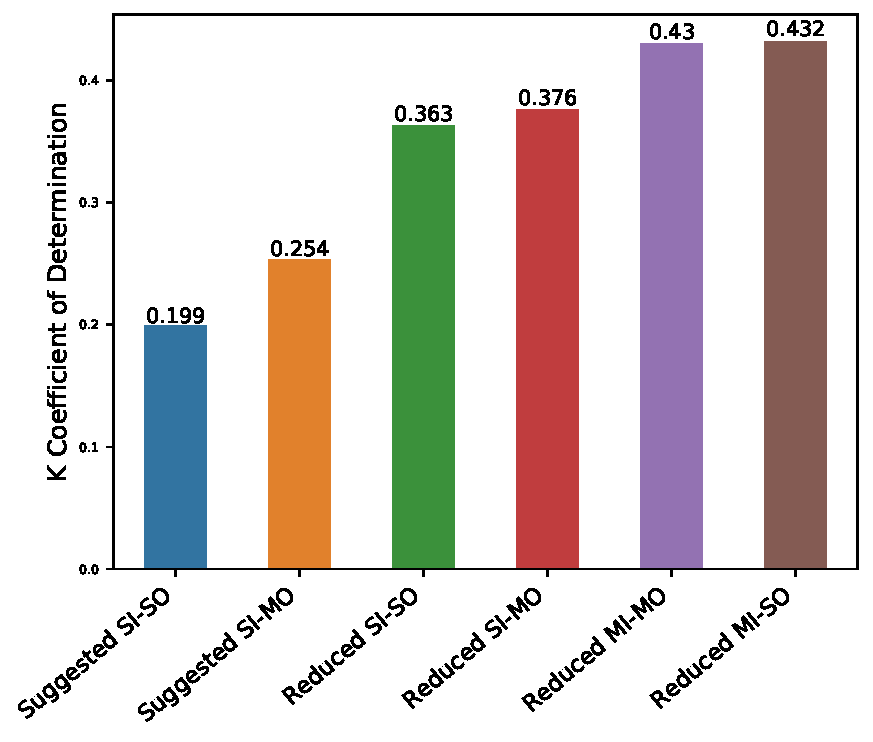
\includegraphics[width=1\linewidth]{RESULTS/BARPLOTS/test_K_determ.pdf}
        \caption{Σύγκριση μοντέλων για την ιδιότητα της περιεκτικότητας του καλίου στο έδαφος}
        \label{fig:K_determ}
    \end{subfigure}
    \begin{subfigure}{0.5\textwidth}
        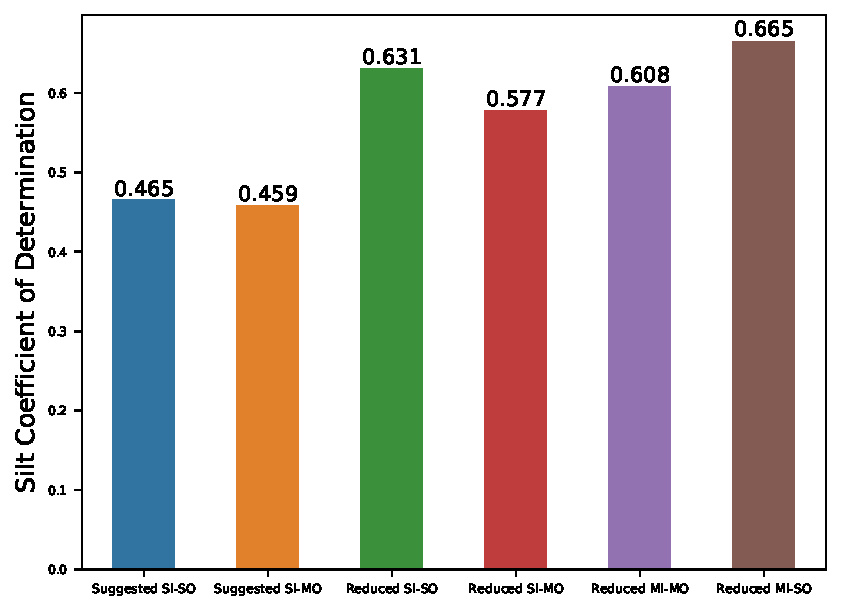
\includegraphics[width=1\linewidth]{RESULTS/BARPLOTS/test_Silt_determ.pdf}
        \caption{Σύγκριση μοντέλων για την ιδιότητα της περιεκτικότητας του εδάφους σε ιλύ}
        \label{fig:Silt_determ}
    \end{subfigure}
    \caption{Ραβδογράμματα συντελεστή προσδιορισμού για τις ιδιότητες \tl{K} και \tl{Silt}}
    \label{fig:barpl-K-Silt}
\end{figure}

Στα ραβδογράμματα των σχημάτων \ref{fig:barpl-OC-CEC} με \ref{fig:barpl-K-Silt} φαίνεται μια πιο ποιοτική απεικόνιση της βελτίωσης που υπάρχει στην επίδοση του βέλτιστου και του προτεινόμενου μοντέλου με την χρήση της μετρικής του συντελεστή προσδιορισμού για κάθε εδαφική ιδιότητα. Αξιοσημείωτη είναι η διαφορά στα διαγράμματα των επιδόσεων στις προβλέψεις του φωσφόρου και του καλίου στα σχήματα \ref{fig:P_determ} και \ref{fig:K_determ} αντίστοιχα. Σημαντική είναι επίσης η βελτίωση της ικανότητας πρόβλεψης της περιεκτικότητας σε άμμο για την οποία παρατηρείται χαμηλός συντελεστής προσδιορισμού στο μοντέλο της προτεινόμενης υλοποίησης όπως φαίνεται στο σχήμα \ref{fig:Sand_determ}.

\section{Οπτικοποίηση συνελικτικών φίλτρων του μοντέλου}
Η φύση των δισδιάστατων νευρωνικών δικτύων τα καθιστά κατάλληλα για πειραματισμούς σχετικά με την μορφή της εισόδου που εισέρχεται στο μοντέλο σε κάθε επίπεδο του. Σε κάποιες περιπτώσεις οι μορφές των συνελικτικών φίλτρων θα μπορούσαν να ερμηνευτούν αναλόγως με τα χαρακτηριστικά που αφορούν την μορφή της εισόδου και την πληροφορία που αποσκοπείται να εξαχθεί από αυτή. Στην περίπτωση της εισόδου των μοντέλων που πραγματεύεται η παρούσα διπλωματική εργασία, τα μοτίβα που ανιχνεύονται στα σπεκτρογράμματα είναι ίσως κάποιες συγκεκριμένες διακυμάνσεις στις φασματικές υπογραφές και στους μετασχηματισμούς \tl{wavelet}.\\

Για την οπτικοποίηση των ενεργοποιήσεων των διαφόρων επιπέδων του μοντέλου εκπαιδεύεται ένα μοντέλο μιας εισόδου και μιας εξόδου, συγκεκριμένα  με τη χρήση φασματικών υπογραφών ανακλαστικότητας και με έξοδο την περιεκτικότητα σε οργανικό άνθρακα. Στη συνέχεια παρατίθενται οι μορφές των εξόδων κάθε επιπέδου από την είσοδο μέχρι το σημείο του μοντέλου όπου τα δεδομένα είναι σε δισδιάστατη μορφή.

\begin{figure}[H]
  \begin{center}
    \includesvg[width=1\textwidth]{RESULTS/model_layer_0_OC_input_3}
    \caption{Είσοδος μετά την μετατροπή σε σπεκτρόγραμμα από φασματική υπογραφή ανακλαστικότητας}
  \end{center}
\end{figure}

%\begin{figure}[htbp]
%    \begin{subfigure}{0.5\textwidth}
        %\includesvg[width=1\linewidth]{RESULTS/model_layer_1_OC_conv2d_4}
        %\caption{Πραγματικές τιμές}
        %\label{fig:subim1}
%    \end{subfigure}
%    \begin{subfigure}{0.5\textwidth}
        %\includesvg[width=1\linewidth]{RESULTS/model_layer_1_OC_conv2d_4_standarized}
        %\caption{Κανονικοποιημένες τιμές}
        %\label{fig:subim1}
%    \end{subfigure}
%    \caption{Μορφή της εξόδου του πρώτου δισδιάστατου συνελικτικού επιπέδου. Έξοδος για τα πρώτα 18 \tl{Feature %Maps}}
%\end{figure}
%
%\begin{figure}[H]
%  \begin{center}
%    \includesvg[width=0.3\textwidth]{RESULTS/model_layer_1_OC_conv2d_4_kernels}
%    \caption{Μορφή των συνελικιτκών φίλτρων που χρησιμοποιήθηκαν από το πρώτο δισδιάστατο συνελικτικό επιπέδο. %Φαίνονται τα  18 πρώτα φίλτρα}
%  \end{center}
%\end{figure}

\begin{figure}[H]
    \begin{subfigure}{0.7\textwidth}
        \begin{subfigure}{\textwidth}
            \includesvg[width=1\linewidth]{RESULTS/model_layer_1_OC_conv2d_4}
            \caption{Πραγματικές τιμές}
            \label{fig:layer_1}
        \end{subfigure}
        \begin{subfigure}{\textwidth}
            \includesvg[width=1\linewidth]{RESULTS/model_layer_1_OC_conv2d_4_standarized}
            \caption{Κανονικοποιημένες τιμές}
            \label{fig:layer_1_stand}
        \end{subfigure}
    \end{subfigure}
    \begin{subfigure}{0.3\textwidth}
        \includesvg[width=\textwidth]{RESULTS/model_layer_1_OC_conv2d_4_kernels}
        \caption{Μορφή των συνελικιτκών φίλτρων που χρησιμοποιήθηκαν από το πρώτο δισδιάστατο συνελικτικό επιπέδο. Φαίνονται τα  18 πρώτα φίλτρα}
        \label{fig:layer_1_filters}
    \end{subfigure}
    \caption{Μορφή της εξόδου του πρώτου δισδιάστατου συνελικτικού επιπέδου. Έξοδος για τα πρώτα 18 \tl{Feature Maps}}
    \label{fig:layer_1_full}
\end{figure}

\begin{figure}[H]
    \begin{subfigure}{0.5\textwidth}
        \includesvg[width=1\linewidth]{RESULTS/model_layer_2_OC_batch_normalization_8}
        \caption{Πραγματικές τιμές}
        \label{fig:layer_2}
    \end{subfigure}
    \begin{subfigure}{0.5\textwidth}
        \includesvg[width=1\linewidth]{RESULTS/model_layer_2_OC_batch_normalization_8_standarized}
        \caption{Κανονικοποιημένες τιμές}
        \label{fig:layer_2_stand}
    \end{subfigure}
    \caption{Μορφή της εξόδου μετά το επίπεδο της κανονικοποίησης παρτίδας. Έξοδος για τα πρώτα 18 \tl{Feature Maps}}
    \label{fig:layer_2_full}
\end{figure}

\begin{figure}[H]
    \begin{subfigure}{0.5\textwidth}
        \includesvg[width=1\linewidth]{RESULTS/model_layer_3_OC_re_lu_8}
        \caption{Πραγματικές τιμές}
        \label{fig:layer_3}
    \end{subfigure}
    \begin{subfigure}{0.5\textwidth}
        \includesvg[width=1\linewidth]{RESULTS/model_layer_3_OC_re_lu_8_standarized}
        \caption{Κανονικοποιημένες τιμές}
        \label{fig:layer_3_stand}
    \end{subfigure}
    \caption{Μορφή της εξόδου του πρώτου δισδιάστατου συνελικτικού επιπέδου μετά την συνάρτηση ενεργοποίησης \tl{ReLU}. Έξοδος για τα πρώτα 18 \tl{Feature Maps}}
    \label{fig:layer_3_full}
\end{figure}

\begin{figure}[H]
    \begin{subfigure}{0.5\textwidth}
        \includesvg[width=1\linewidth]{RESULTS/model_layer_4_OC_max_pooling2d_2}
        \caption{Πραγματικές τιμές}
        \label{fig:layer_4}
    \end{subfigure}
    \begin{subfigure}{0.5\textwidth}
        \includesvg[width=1\linewidth]{RESULTS/model_layer_4_OC_max_pooling2d_2_standarized}
        \caption{Κανονικοποιημένες τιμές}
        \label{fig:layer_4_stand}
    \end{subfigure}
    \caption{Μορφή της εξόδου μετά την συνάρτηση ενεργοποίησης \tl{ReLU} του πρώτου επιπέδου και της εφαρμογής συγκέντρωσης μεγίστων. Έξοδος για τα πρώτα 18 \tl{Feature Maps}}
    \label{fig:layer_4_full}
\end{figure}


\begin{figure}[H]
    \begin{subfigure}{0.7\textwidth}
        \begin{subfigure}{\textwidth}
            \includesvg[width=1\linewidth]{RESULTS/model_layer_5_OC_conv2d_5}
            \caption{Πραγματικές τιμές}
            \label{fig:layer_5}
        \end{subfigure}
        \begin{subfigure}{\textwidth}
            \includesvg[width=1\linewidth]{RESULTS/model_layer_5_OC_conv2d_5_standarized}
            \caption{Κανονικοποιημένες τιμές}
            \label{fig:layer_5_stand}
        \end{subfigure}
    \end{subfigure}
    \begin{subfigure}{0.3\textwidth}
        \includesvg[width=\textwidth]{RESULTS/model_layer_5_OC_conv2d_5_kernels}
        \caption{Μορφή των συνελικιτκών φίλτρων που χρησιμοποιήθηκαν από το δεύτερο δισδιάστατο συνελικτικό επιπέδο. Φαίνονται τα  18 πρώτα φίλτρα}
        \label{fig:layer_5_filters}
    \end{subfigure}
    \caption{Μορφή της εξόδου του δευτερου δισδιάστατου συνελικτικού επιπέδου. Έξοδος για τα πρώτα 18 \tl{Feature Maps}}
    \label{fig:layer_5_full}
\end{figure}

%\begin{figure}[htbp]
    %\begin{subfigure}{0.5\textwidth}
        %\includesvg[width=1\linewidth]{RESULTS/model_layer_5_OC_conv2d_5}
        %\caption{Πραγματικές τιμές}
        %\label{fig:subim7}
    %\end{subfigure}
    %\begin{subfigure}{0.5\textwidth}
        %\includesvg[width=1\linewidth]{RESULTS/model_layer_5_OC_conv2d_5_standarized}
        %\caption{Κανονικοποιημένες τιμές}
        %\label{fig:subim8}
    %\end{subfigure}
    %\caption{Μορφή της εξόδου του δευτερου δισδιάστατου συνελικτικού επιπέδου. Έξοδος για τα πρώτα 18 %\tl{Feature Maps}}
%\end{figure}
%
%\begin{figure}[H]
  %\begin{center}
%    \includesvg[width=0.3\textwidth]{RESULTS/model_layer_5_OC_conv2d_5_kernels}
%    \caption{Μορφή των συνελικιτκών φίλτρων που χρησιμοποιήθηκαν από το δεύτερο δισδιάστατο συνελικτικό επιπέδο. Φαίνονται τα  18 πρώτα φίλτρα}
  %\end{center}
%\end{figure}

\begin{figure}[H]
    \begin{subfigure}{0.5\textwidth}
        \includesvg[width=1\linewidth]{RESULTS/model_layer_6_OC_batch_normalization_9}
        \caption{Πραγματικές τιμές}
        \label{fig:layer_6}
    \end{subfigure}
    \begin{subfigure}{0.5\textwidth}
        \includesvg[width=1\linewidth]{RESULTS/model_layer_6_OC_batch_normalization_9_standarized}
        \caption{Κανονικοποιημένες τιμές}
        \label{fig:layer_6_stand}
    \end{subfigure}
    \caption{Μορφή της εξόδου μετά το επίπεδο της κανονικοποίησης παρτίδας του δεύτερου συνελικτικού επιπέδου. Έξοδος για τα πρώτα 18 \tl{Feature Maps}}
    \label{fig:layer_6_full}
\end{figure}

\begin{figure}[H]
    \begin{subfigure}{0.5\textwidth}
        \includesvg[width=1\linewidth]{RESULTS/model_layer_7_OC_re_lu_9}
        \caption{Πραγματικές τιμές}
        \label{fig:layer_7}
    \end{subfigure}
    \begin{subfigure}{0.5\textwidth}
        \includesvg[width=1\linewidth]{RESULTS/model_layer_7_OC_re_lu_9_standarized}
        \caption{Κανονικοποιημένες τιμές}
        \label{fig:layer_7_stand}
    \end{subfigure}
    \caption{Μορφή της εξόδου του δεύτερου δισδιάστατου συνελικτικού επιπέδου μετά την συνάρτηση ενεργοποίησης \tl{ReLU}. Έξοδος για τα πρώτα 18 \tl{Feature Maps}}
    \label{fig:layer_7_full}
\end{figure}

Στις παραπάνω εικόνες φαίνεται ο τρόπος με τον οποίο ένα μοντέλο το οποίο έχει προηγουμένως εκπαιδευτεί, επεξεργάζεται την μονοκαναλική εικόνα εισόδου σε όλα τα επίπεδα τα οποία έχει δισδιάστατη μορφή.\\

Στα δισδιάστατα συνελικτικά επίπεδα των σχημάτων \ref{fig:layer_1_full} και \ref{fig:layer_5_full} παρατηρείται πως η εικόνα εισόδου τροποποιείται σε διαφορετικές εκδοχές της ανάλογα με το συνελικτικό φίλτρο που εφαρμόζεται.\\

Στα επίπεδα κανονικοποίησης παρτίδας των σχημάτων \ref{fig:layer_2_full} και \ref{fig:layer_6_full} είναι ορατή η κανονικοποίηση που υφίσταται το σύνολο των \tl{Feature Maps} σε σχέση με το εύρος τιμών που είχαν στα συνελικτικά επίπεδα.\\

Στα επίπεδα ενεργοποίησης με χρήση ανορθωμένης γραμμικής συνάρτησης \tl{ReLU}, τα οποία απεικονίζονται στα σχήματα \ref{fig:layer_3_full} και \ref{fig:layer_7_full}, φαίνεται πως η εφαρμογή της συνάρτησης ενεργοποίησης επιτρέπει μόνο στα μέρη των εικόνων με μεγαλύτερες τιμές, τα οποία πιθανώς περιέχουν χρήσιμη πληροφορία, να μεταφερθούν προς το επόμενο επίπεδο.\\

Το επίπεδα συγκέντρωσης μεγίστων, του οποίου η έξοδος φαίνεται στο σχήμα \ref{fig:layer_4_full}, τροποποιεί την είσοδο τους μειώνοντας τις διαστάσεις της ενώ διατηρούν τα μέγιστα των περιοχών τις οποίες συγκεντρώνουν. Το αποτέλεσμα οπτικά φαίνεται σαν μια σμίκρυνση της εικόνας εισόδου.\\

Κατά την επεξεργασία της εισόδου από το δισδιάστατο συνελικτικό νευρωνικό δίκτυο η μορφή της εικόνας τροποποιείται σημαντικά με αποτέλεσμα μετά το συνελικτικό επίπεδο 5 του σχήματος \ref{fig:layer_5_full}, η εικόνα να μην έχει καμία ομοιότητα με την αρχική της μορφή.
\chapter{Συμπεράσματα και μελλοντικές επεκτάσεις}
\label{ch:conclusions}
\section{Συμπεράσματα}
Στην παρούσα διπλωματική εργασία έγινε η ανάλυση της λειτουργίας των δισδιάστατων συνελικτικών νευρωνικών δικτύων και της εφαρμογής τους στο πρόβλημα της φασματοσκοπία εδάφους. Μετά από ανάλυση μιας προτεινόμενης υλοποίησης εξετάστηκαν μέθοδοι για την βελτίωση της και την εύρεση ενός βέλτιστου μοντέλου το οποίο θα είναι ικανό να παράγει αξιόλογες προβλέψεις με απλοποιημένη αρχιτεκτονική δομή. Όπως φαίνεται η επίτευξη του παραπάνω είναι εφικτή και οι επιδόσεις των μοντέλων στα οποία καταλήξαμε έχουν σημαντικά καλύτερες επιδόσεις από τα προτεινόμενα.

\section{Επεκτάσεις}
Ορισμένα θέματα που θα μπορούσαν να διερευνηθούν περαιτέρω σχετικά με το αντικείμενο της παρούσας διπλωματικής εργασίας είναι, η διαπίστωση της σημασίας των διαστάσεων της εικόνας και της συσχέτισης της με τις διαστάσεις των συνελικτικών φίλτρων αλλά και την παράμετρο της υποδειγματοληψίας των φασματικών υπογραφών. Επίσης θα μπορούσε να βρεθεί κάποιος διαφορετικός μετασχηματισμός ή μέθοδος για την αναπαράσταση της φασματικής υπογραφής σε δισδιάστατη μορφή, με σκοπό την αποτύπωση κάποιας επιπλέον χρήσιμης πληροφορίας για το σήμα εισόδου.

\appendix
\chapter{Ακρωνύμια και συντομογραφίες}

\selectlanguage{english}
\begin{description}
  \item[CNN] Convolutional Neural Network
\end{description}
\selectlanguage{greek}
\selectlanguage{english}
\begin{description}
  \item[RMSE] Root Mean Square Error
\end{description}
\selectlanguage{greek}


\selectlanguage{english}

\bibliographystyle{IEEEtran}
\bibliography{IEEEabrv,references}

\end{document}